% !TEX root = thesis.tex
\section{Systematic uncertainties}
%{\color{red} Extend Systematics}
\label{sec:systematicerrors}
The main systematic uncertainties in this analysis come from the background estimation, the unfolding procedure and uncertainty in the tracking efficiency. The systematics in background estimation were studied using an alternative method to extract the background, the random background method and the uncertainty in tracking was studied by varying tracking efficiencies in a \pythia~simulation.%The resulting uncertainty is below 5\% for the wide component RMS and below 9\% for the narrow component RMS. 

The systematic uncertainty that arises from the unfolding procedure is estimated by performing the unfolding with two separate methods. Data corrected by the iterative unfolding method are used as the results and the SVD unfolding method is employed to estimate the uncertainty. In a \textsc{Pythia} closure test the true distribution was in general found to be between the unfolded distributions from the iterative and SVD method. The difference between the methods when unfolding data should give a reasonable estimate of the unfolding uncertainty. The resulting uncertainty is below 8\% for both wide and narrow component RMS.



  
 \subsection{Background}
The uncertainty coming from background calculation is estimated by subtracting the background separately for the perpendicular cone and random background methods. Comparisons of the resulting signal distributions are shown in Figure~\ref{fig:signalbg}. 
 
% \begin{figure}[htb]
%\centering
%\begin{subfigure}{0.95\textwidth}
%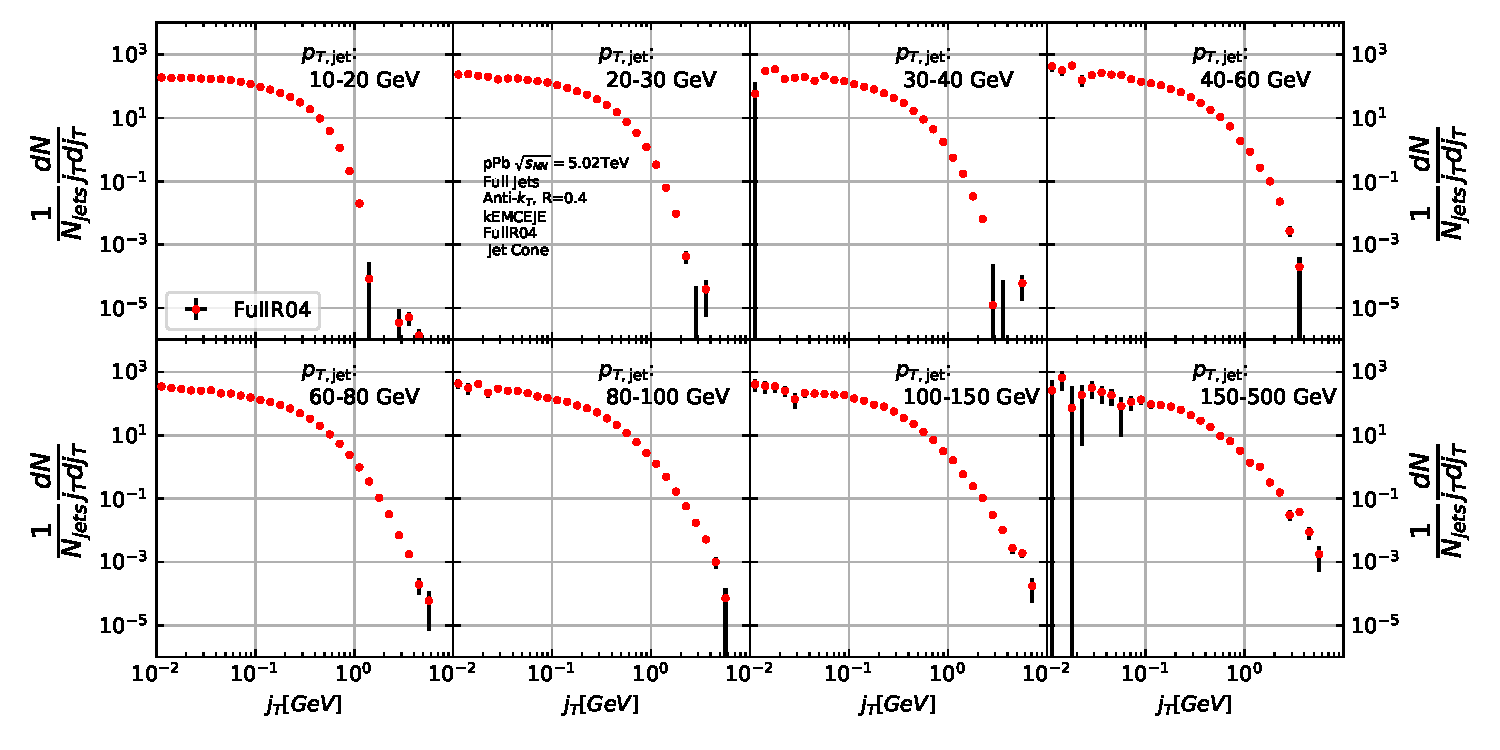
\includegraphics[width=\textwidth]{results/MixedFullJetsR04JetConeJtSignal.pdf}
%%Tag 20170810 python2.7 Python/DrawSignal.py legotrain_CF_pPb-1053_20170223-2002_LHC13bcde.root
%\end{subfigure}
%\caption{$\jt{}$ signal with background subtracted}
%\label{fig:signal}
%\end{figure}

 
Fits are then performed on both perpendicular cone and random background signals. Difference between them is taken as the systematic uncertainty. The fits for individual bins from the random background method are shown in Figure~\ref{fig:fitsrandombg}. Resulting differences between the methods for different components are shown in Figure~\ref{fig:systbg}. The dotted lines are put at $\pm \unit[5]{\%}$ for the narrow component and at $\pm \unit[8]{\%}$ for the wide component. These are taken as systematic estimates for the entire $\pt{,jet}$ range.

\begin{figure}[htb]
\centering
\begin{subfigure}{0.95\textwidth}
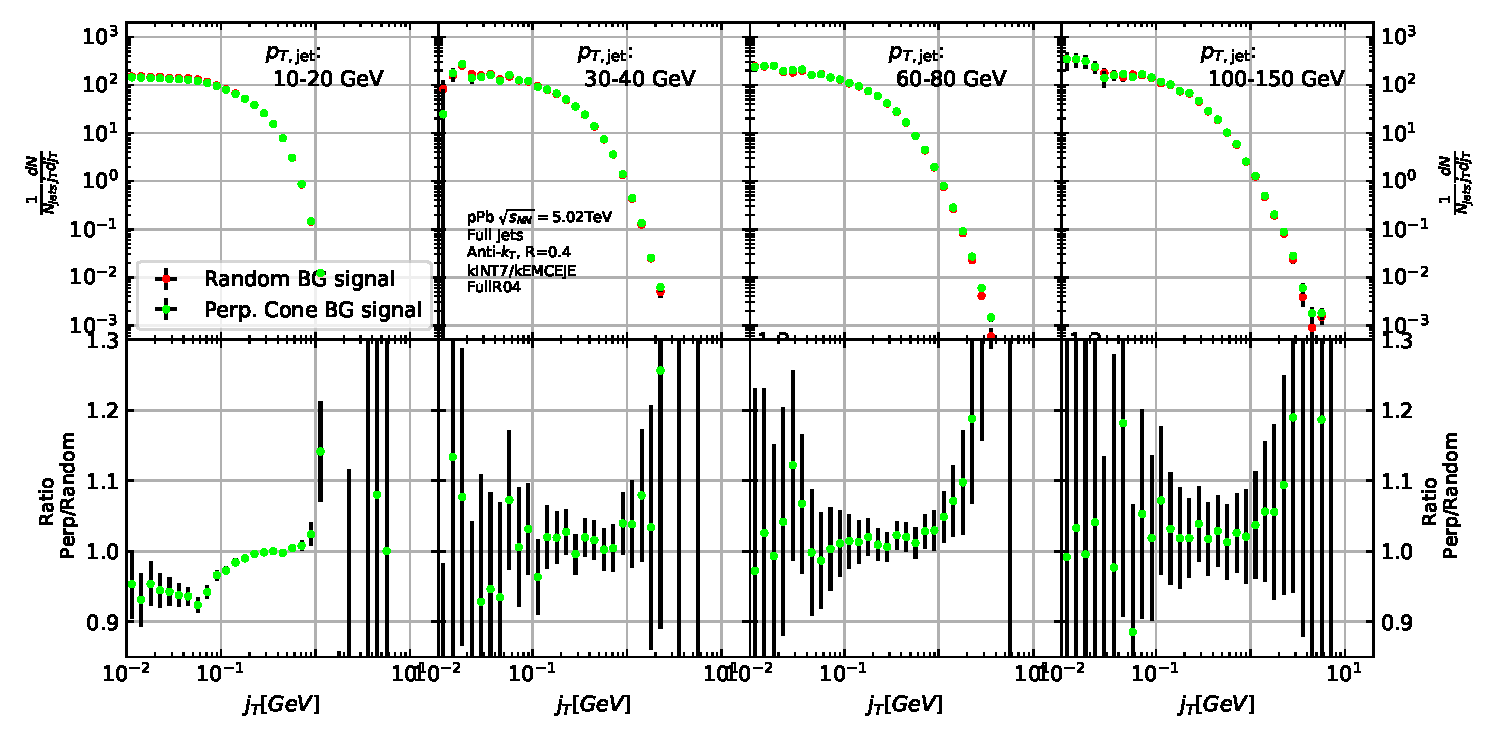
\includegraphics[width=\textwidth]{results/MixedFullJetsR04SignalBackgroundComparison.pdf}
%Tag 20170810 python2.7 Python/DrawSignal.py legotrain_CF_pPb-1053_20170223-2002_LHC13bcde.root
\end{subfigure}
\caption{Comparison of the effect of background method on $\jt{}$ signal}
\label{fig:signalbg}
\end{figure}


\begin{figure}
\centering
%\begin{subfigure}{0.24\textwidth}
%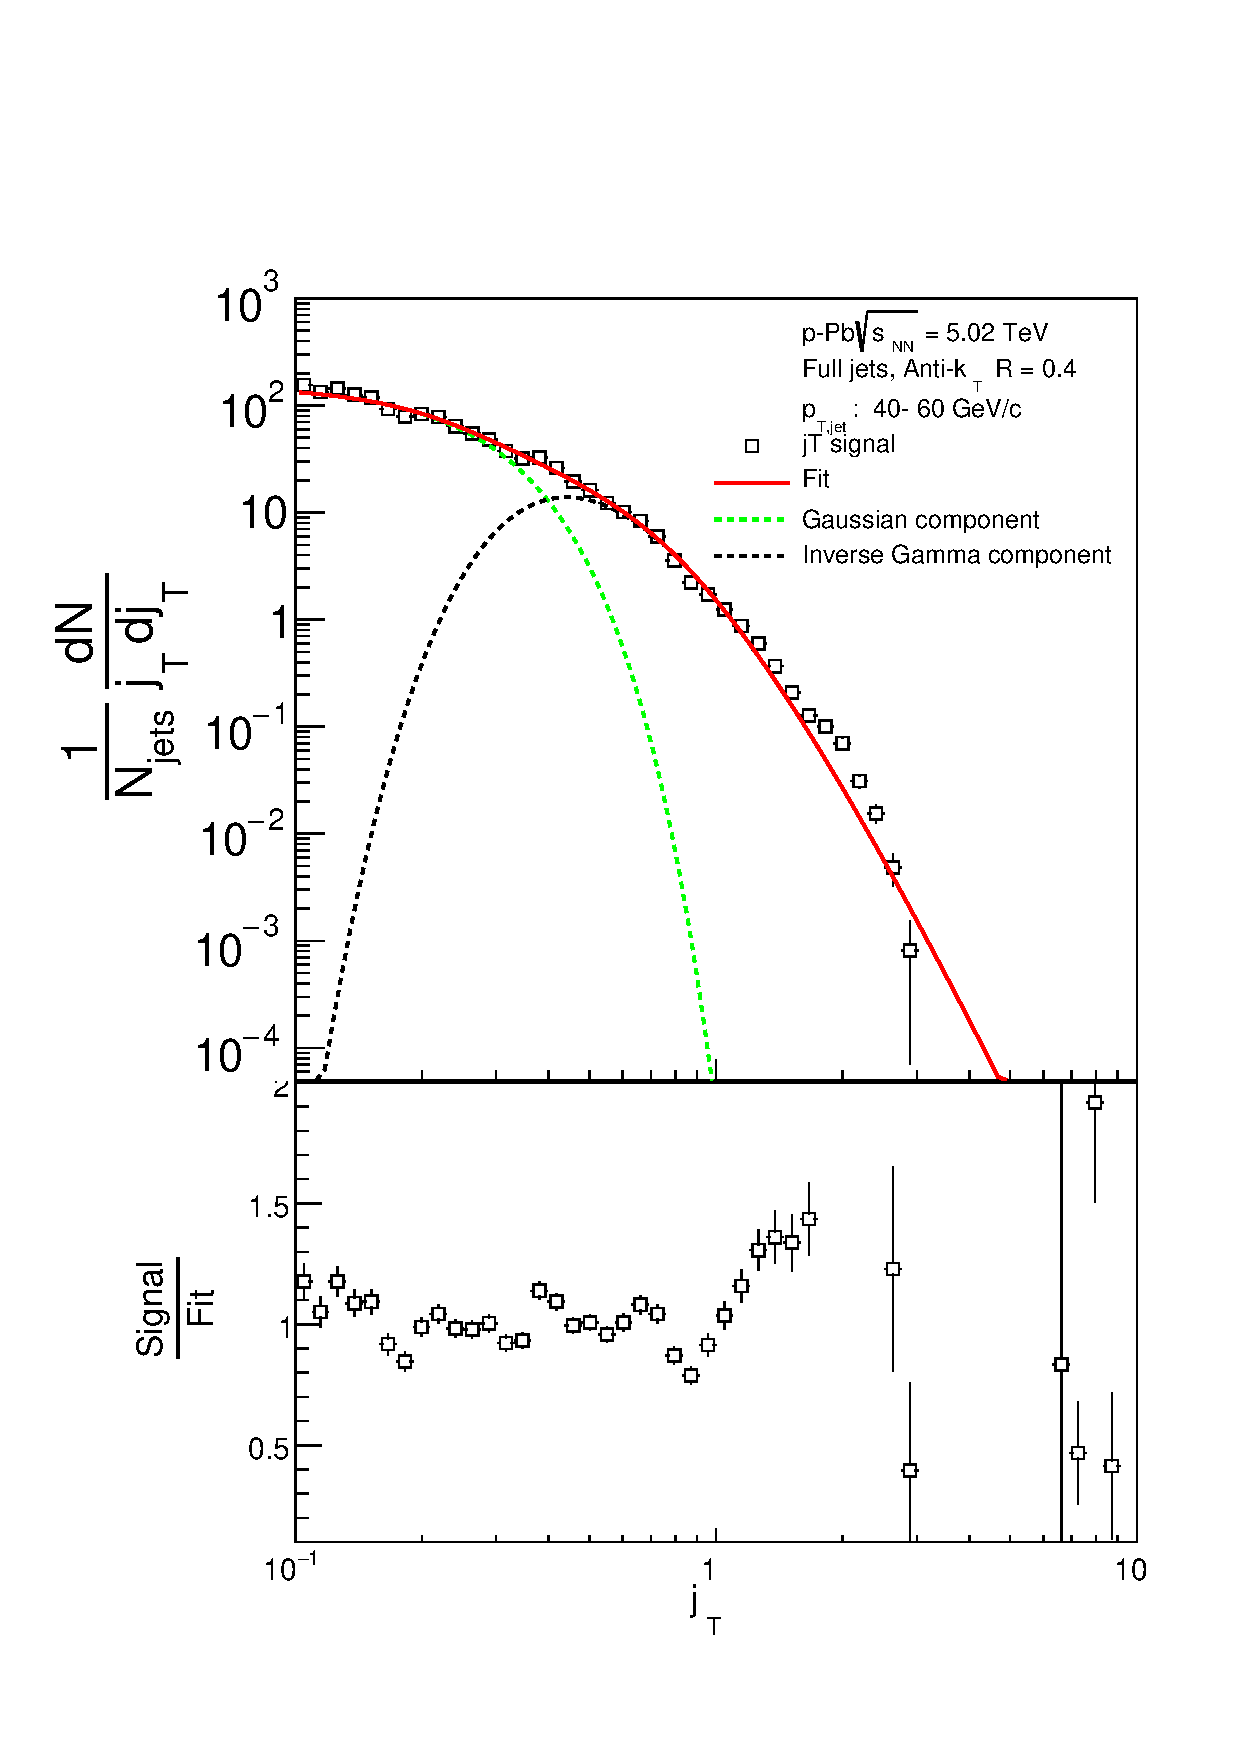
\includegraphics[width=0.95\textwidth]{results/JetConejTSignalFit/JetConejTSignalFitNFin00JetPt04randomBgBayes}
%\end{subfigure}
\begin{subfigure}{0.44\textwidth}
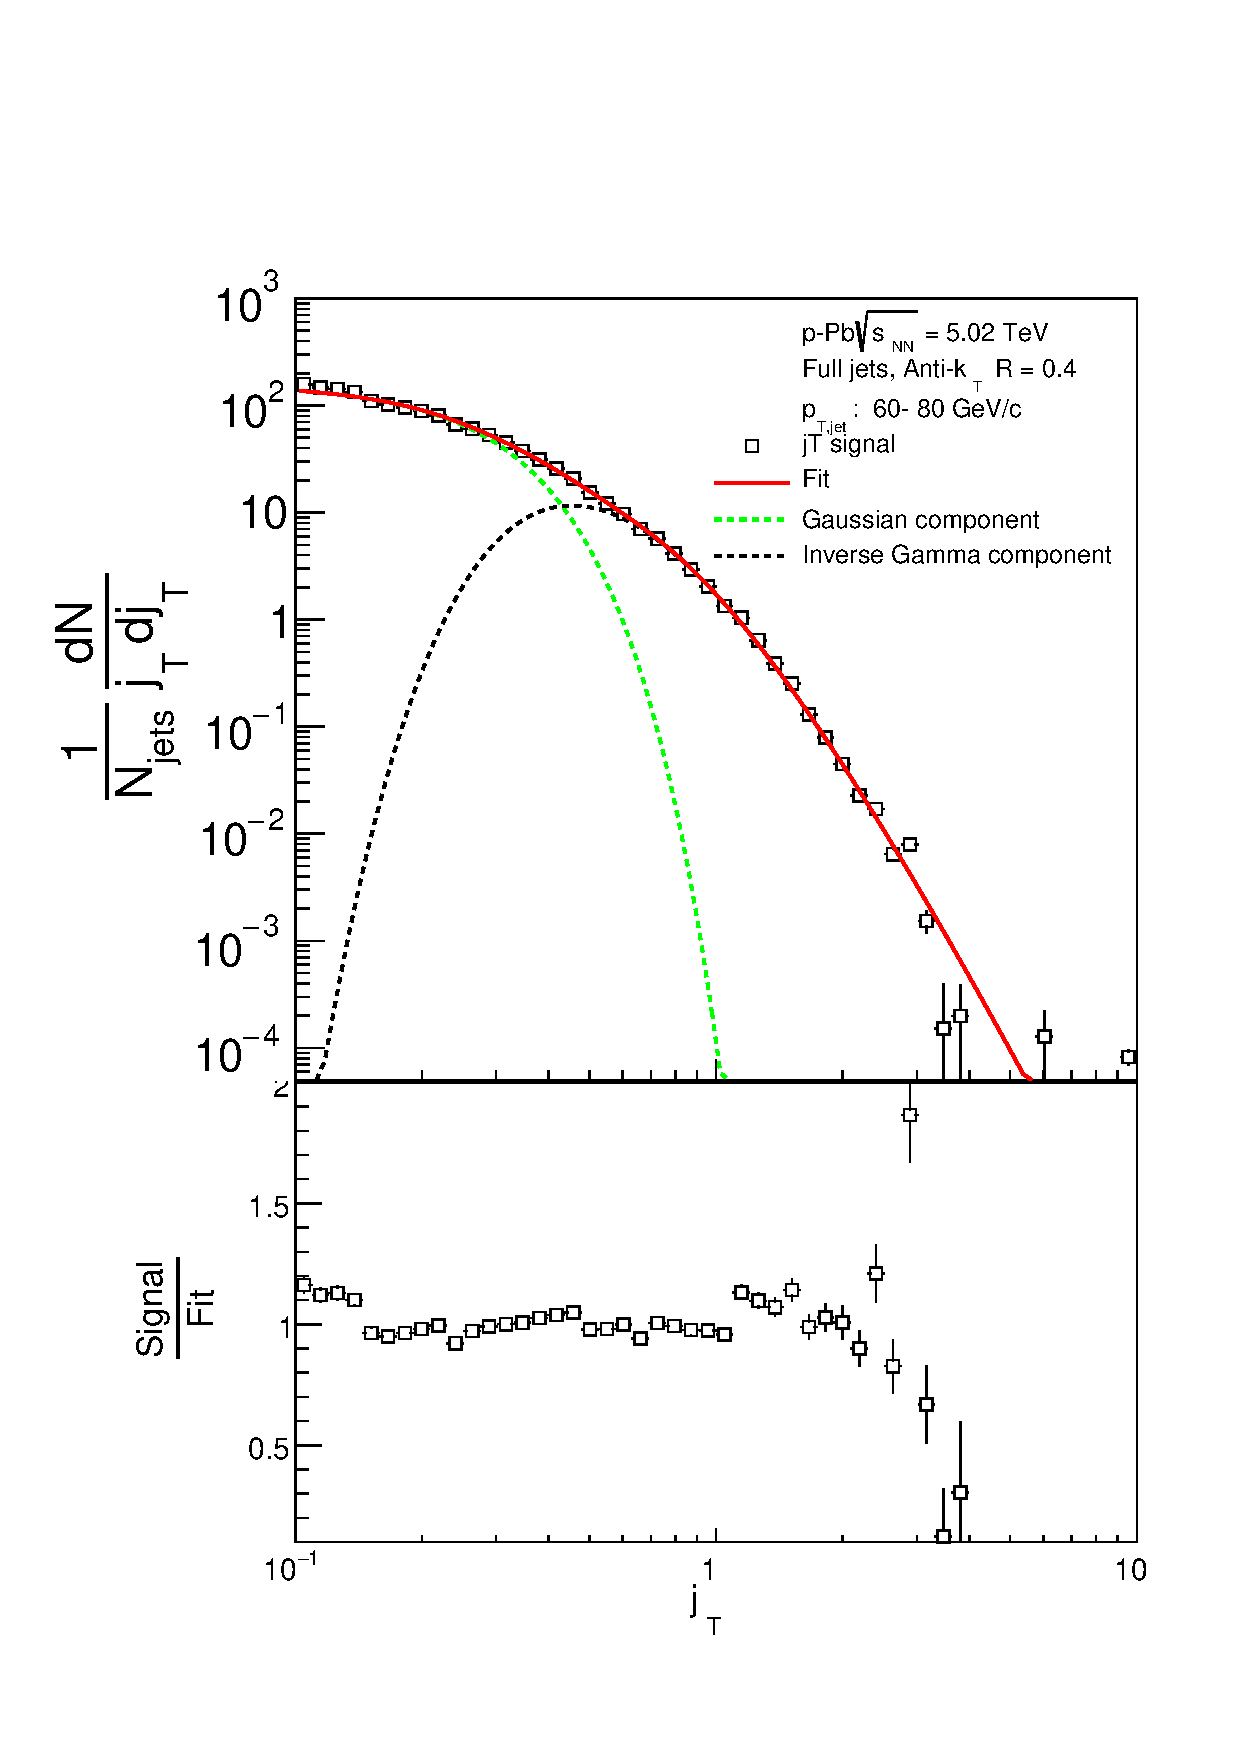
\includegraphics[width=0.95\textwidth]{results/JetConejTSignalFit/JetConejTSignalFitNFin00JetPt05randomBgBayes}
\end{subfigure}
\begin{subfigure}{0.44\textwidth}
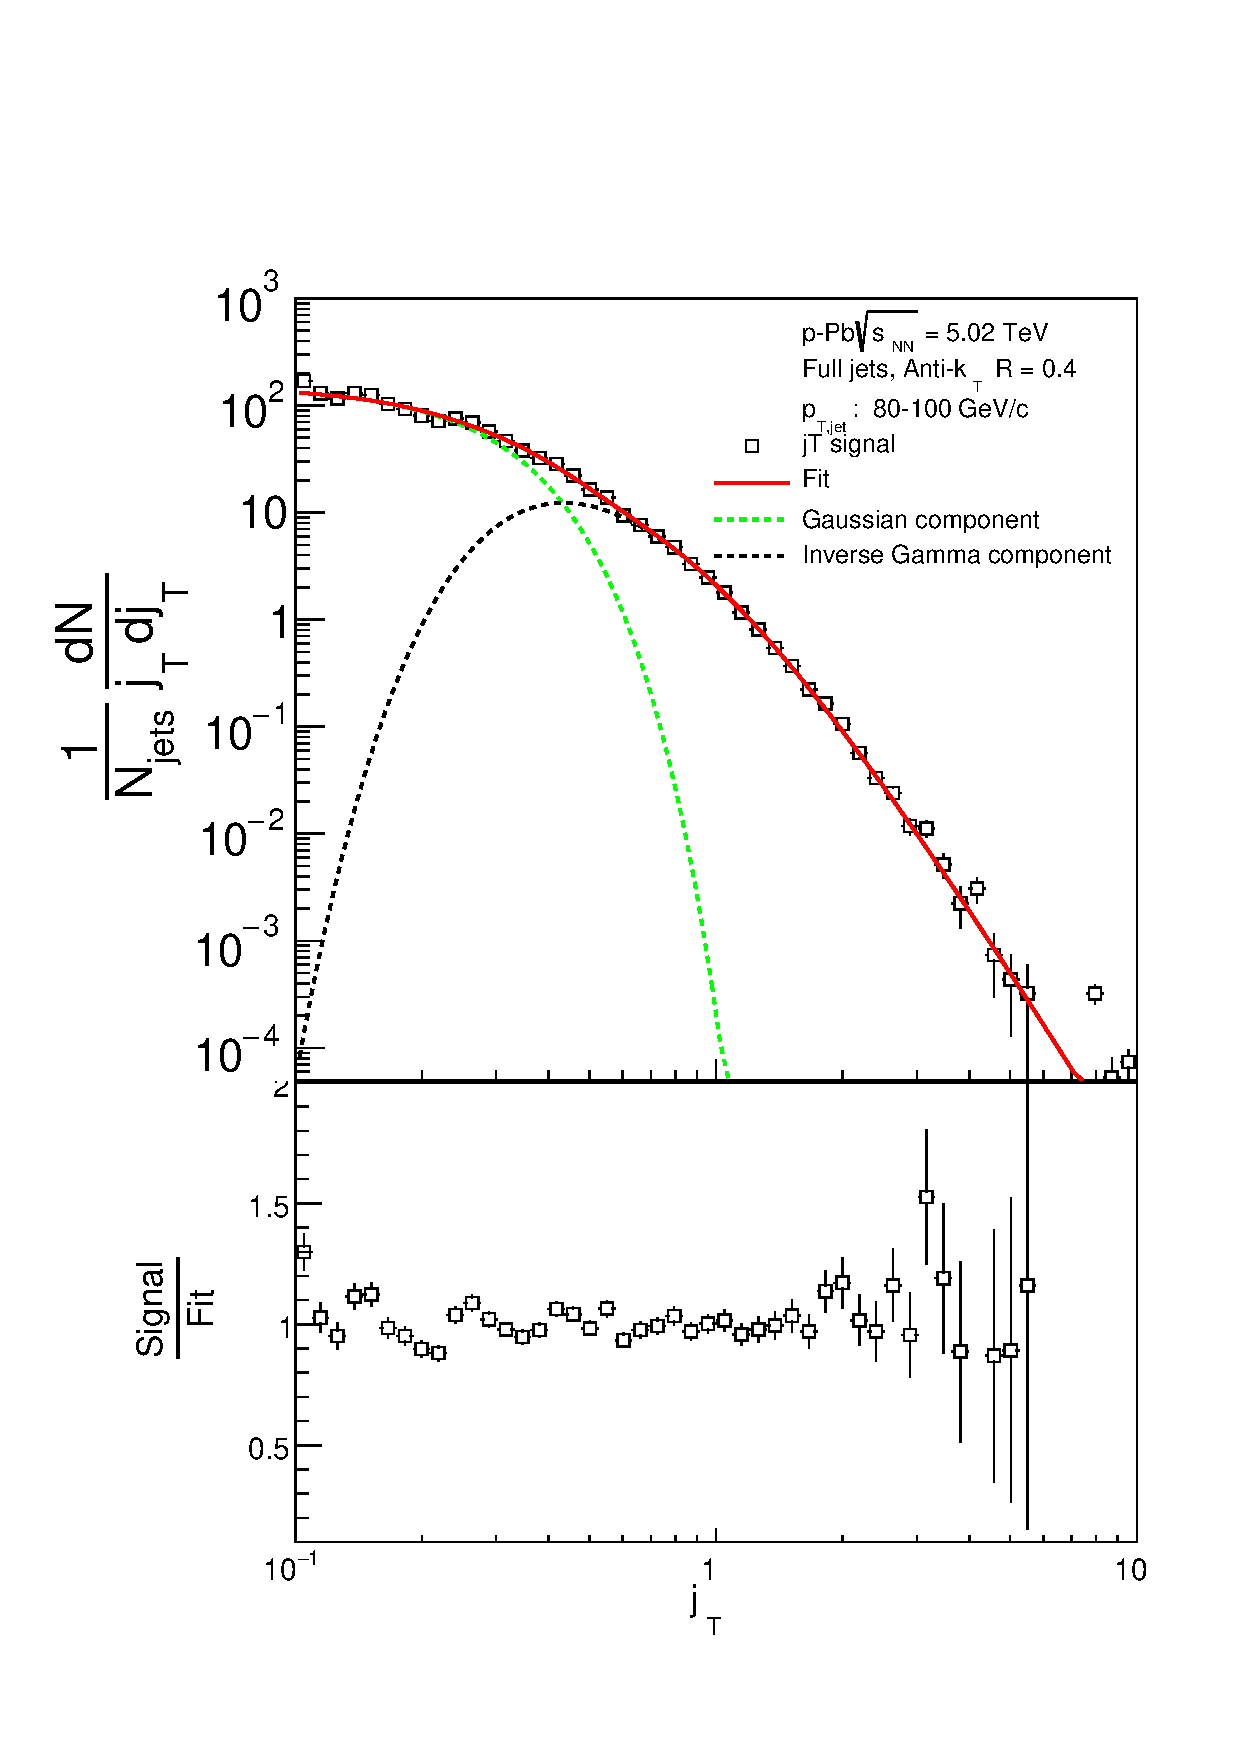
\includegraphics[width=0.95\textwidth]{results/JetConejTSignalFit/JetConejTSignalFitNFin00JetPt06randomBgBayes}
\end{subfigure}
%\begin{subfigure}{0.24\textwidth}
%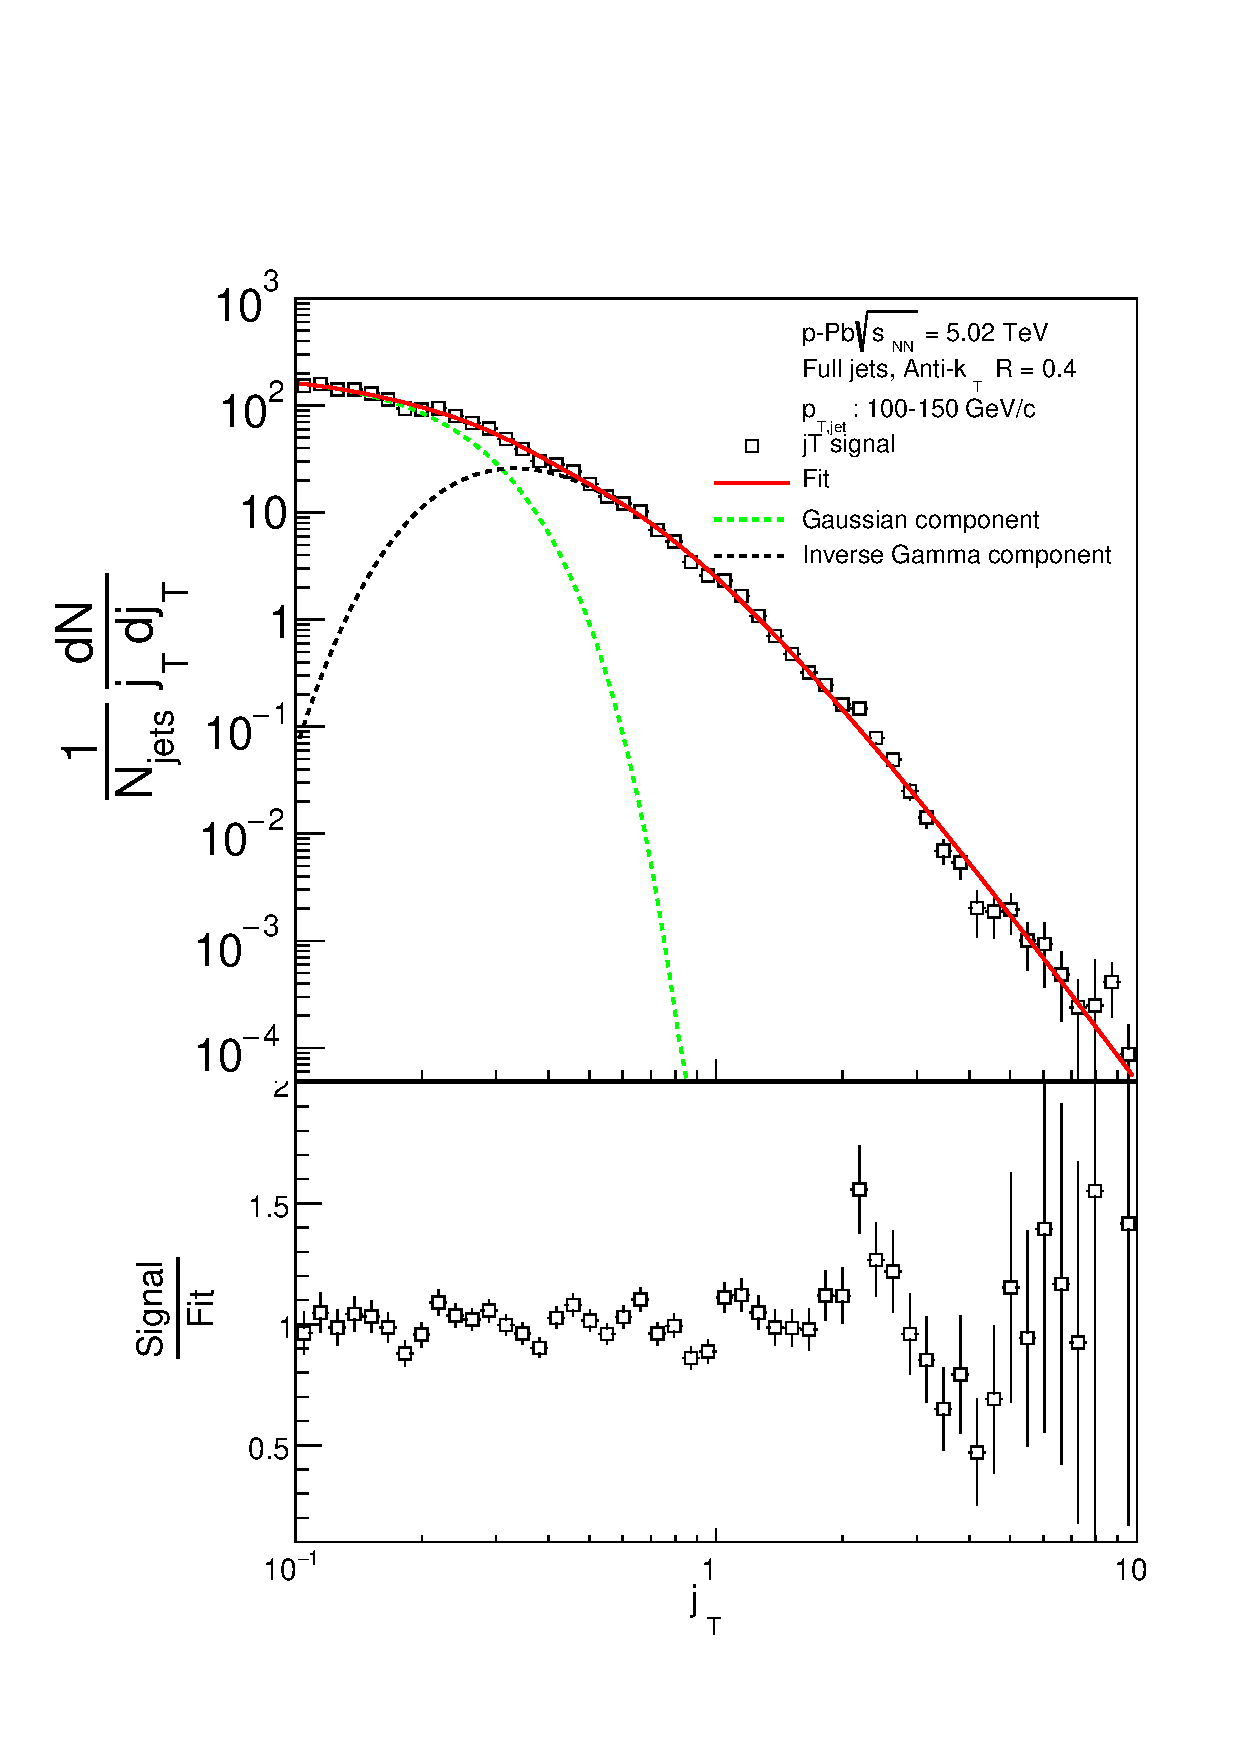
\includegraphics[width=0.95\textwidth]{results/JetConejTSignalFit/JetConejTSignalFitNFin00JetPt07randomBgBayes}
%\end{subfigure}
\caption{$\jt{}$ signal with random background subtraction fits in different jet $\pt{}$ bins}
\label{fig:fitsrandombg}
\end{figure}

\begin{figure}
\centering
\begin{subfigure}{0.44\textwidth}
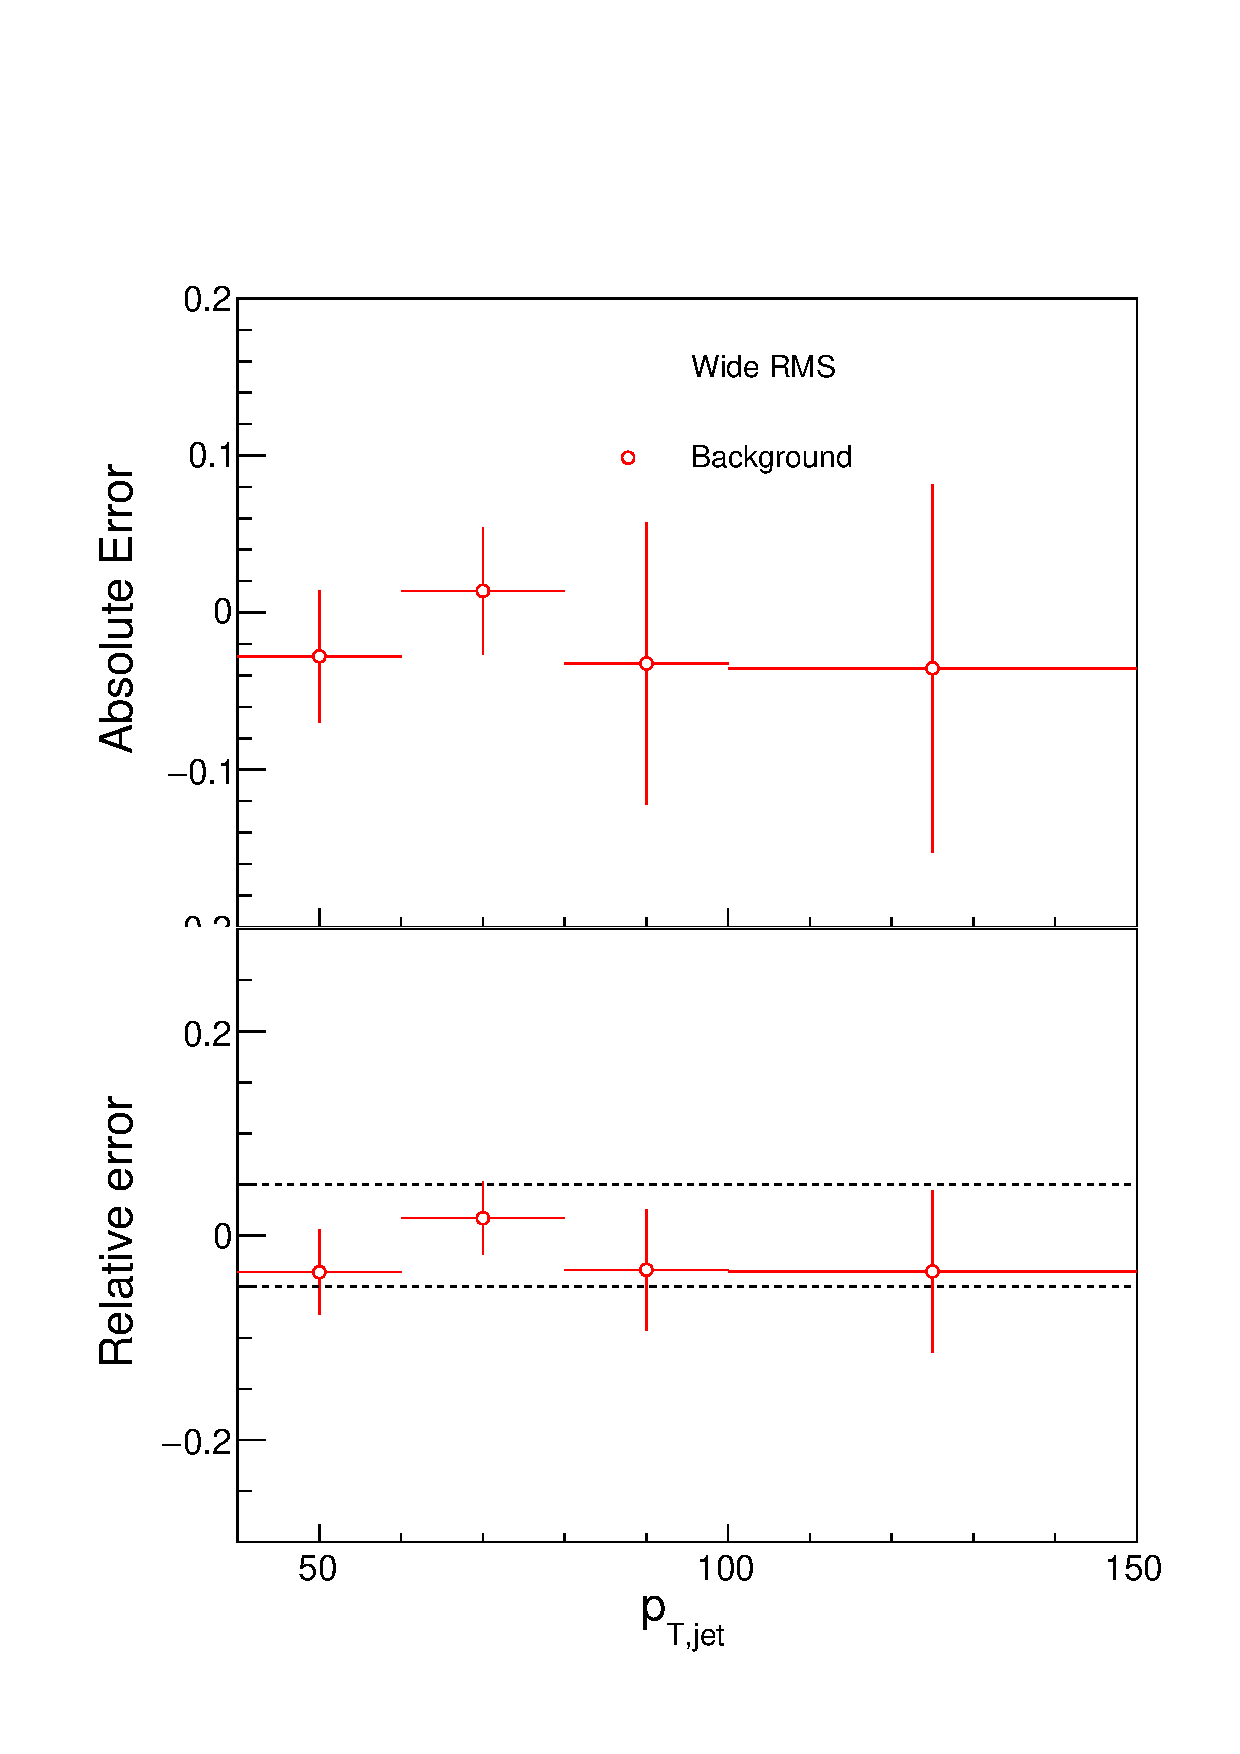
\includegraphics[width=0.95\textwidth]{results/SystematicErrors/SystematicErrorsGammaRMS_BgNFin00JetPt08_linx_data}
\end{subfigure}
\begin{subfigure}{0.44\textwidth}
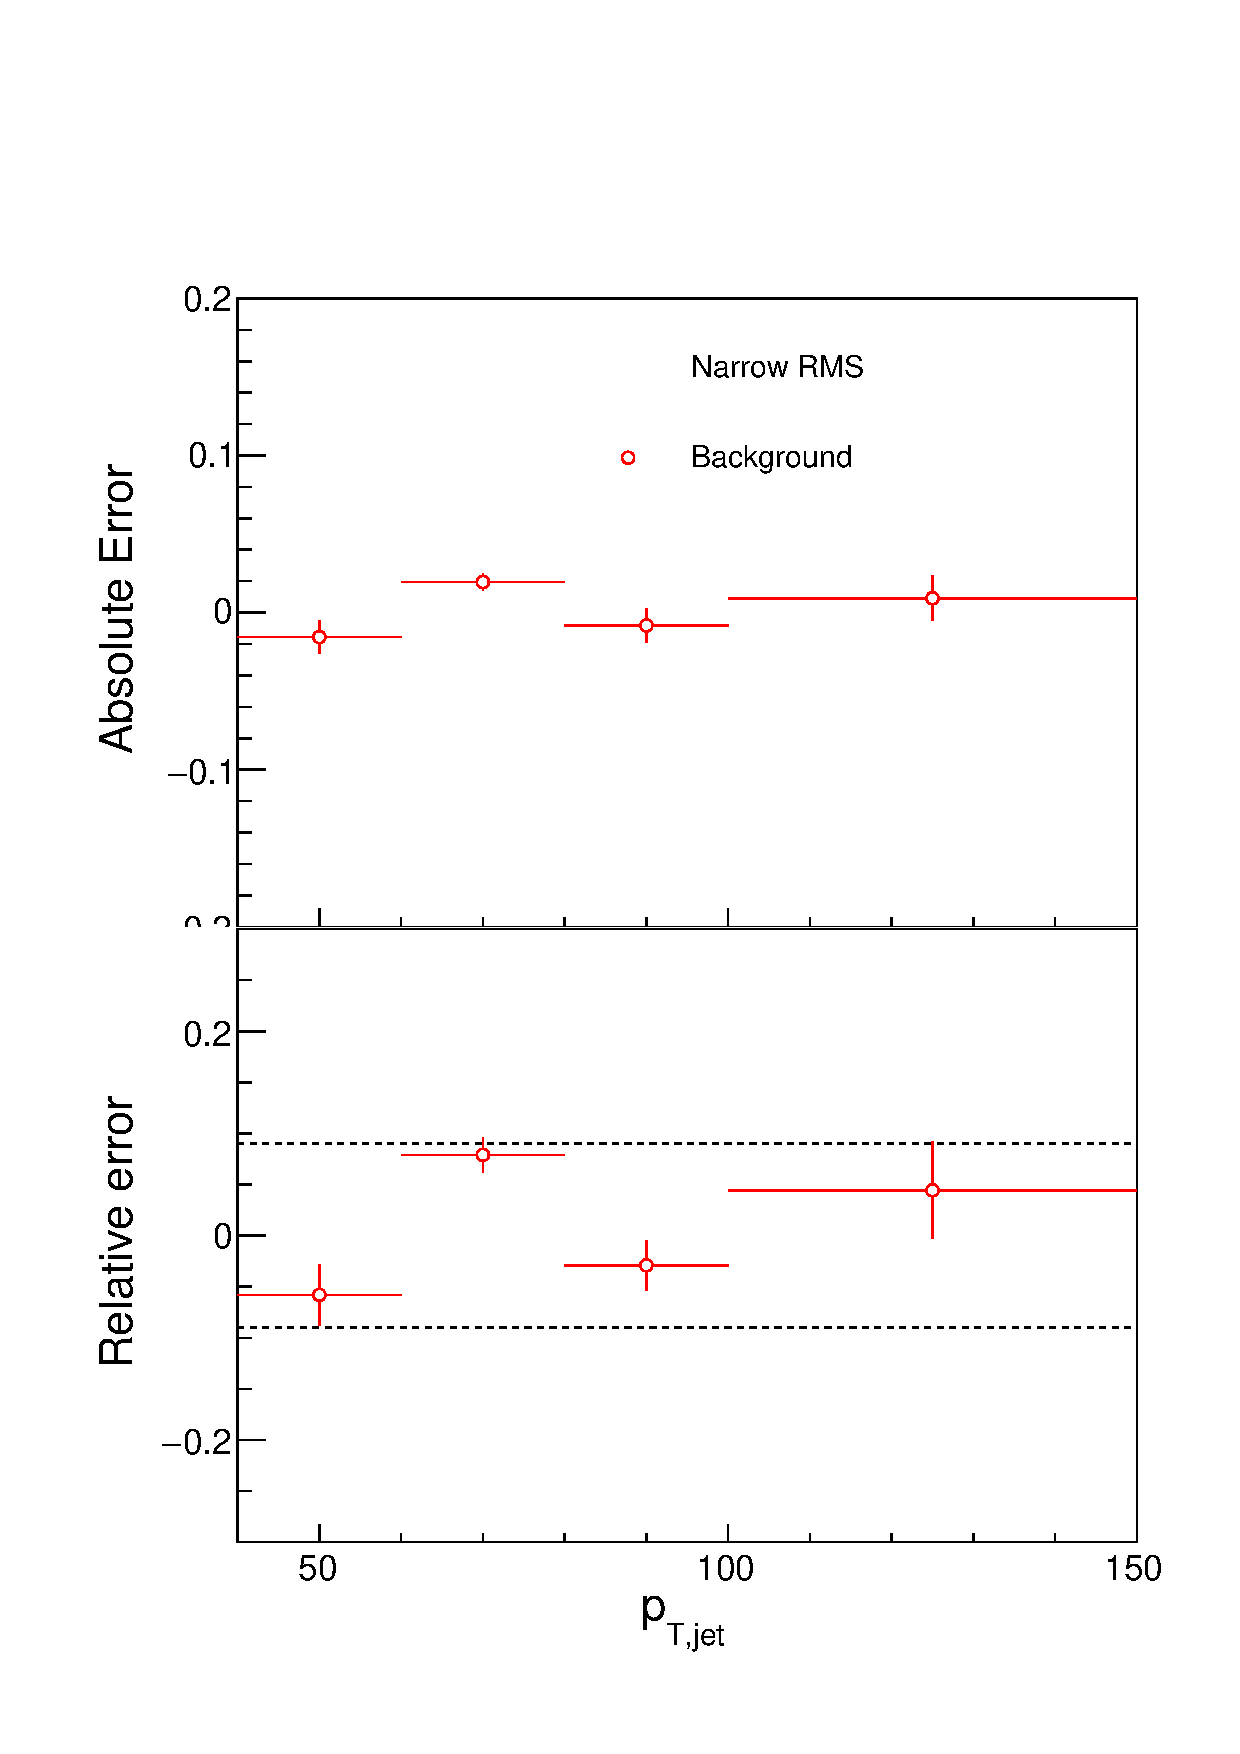
\includegraphics[width=0.95\textwidth]{results/SystematicErrors/SystematicErrorsGausRMS_BgNFin00JetPt08_linx_data}
\end{subfigure}
\caption{Differences between perpendicular cone and random background subtraction in the resulting RMS values}
\label{fig:systbg}
\end{figure}

  
  
  
  \subsection{Unfolding}
Unfolding is the second major source of systematic uncertainty. To estimate the uncertainty related to the unfolding procedure several checks are performed. The main systematic uncertainty estimation comes from comparing results performed using both SVD and Bayesian unfolding. Difference between the methods is taken as the systematic uncertainty. Since SVD unfolding does not have a two dimensional option, the unfolding is done bin by bin. %The resulting distributions after SVD unfolding and background subtraction with the perpendicular cone method are shown in Figure~\ref{fig:fitsSVD}. 

As in the background systematic estimation, fits are performed for both cases separately. Resulting differences between the methods for different components are shown in Figure~\ref{fig:systunf}. The dotted lines are at $\pm \unit[8]{\%}$ for both components. These are taken to be the systematic uncertainty related to unfolding. 

%\begin{figure}
%\centering
%\caption{Resulting signal distributions from SVD unfolding with the perpendicular cone background methods. These are compared to the results from the Bayesian algorithm to estimate the systematic uncertainty.}
%\label{fig:fitsSVD}
%\end{figure}


\begin{figure}
\centering
\begin{subfigure}{0.44\textwidth}
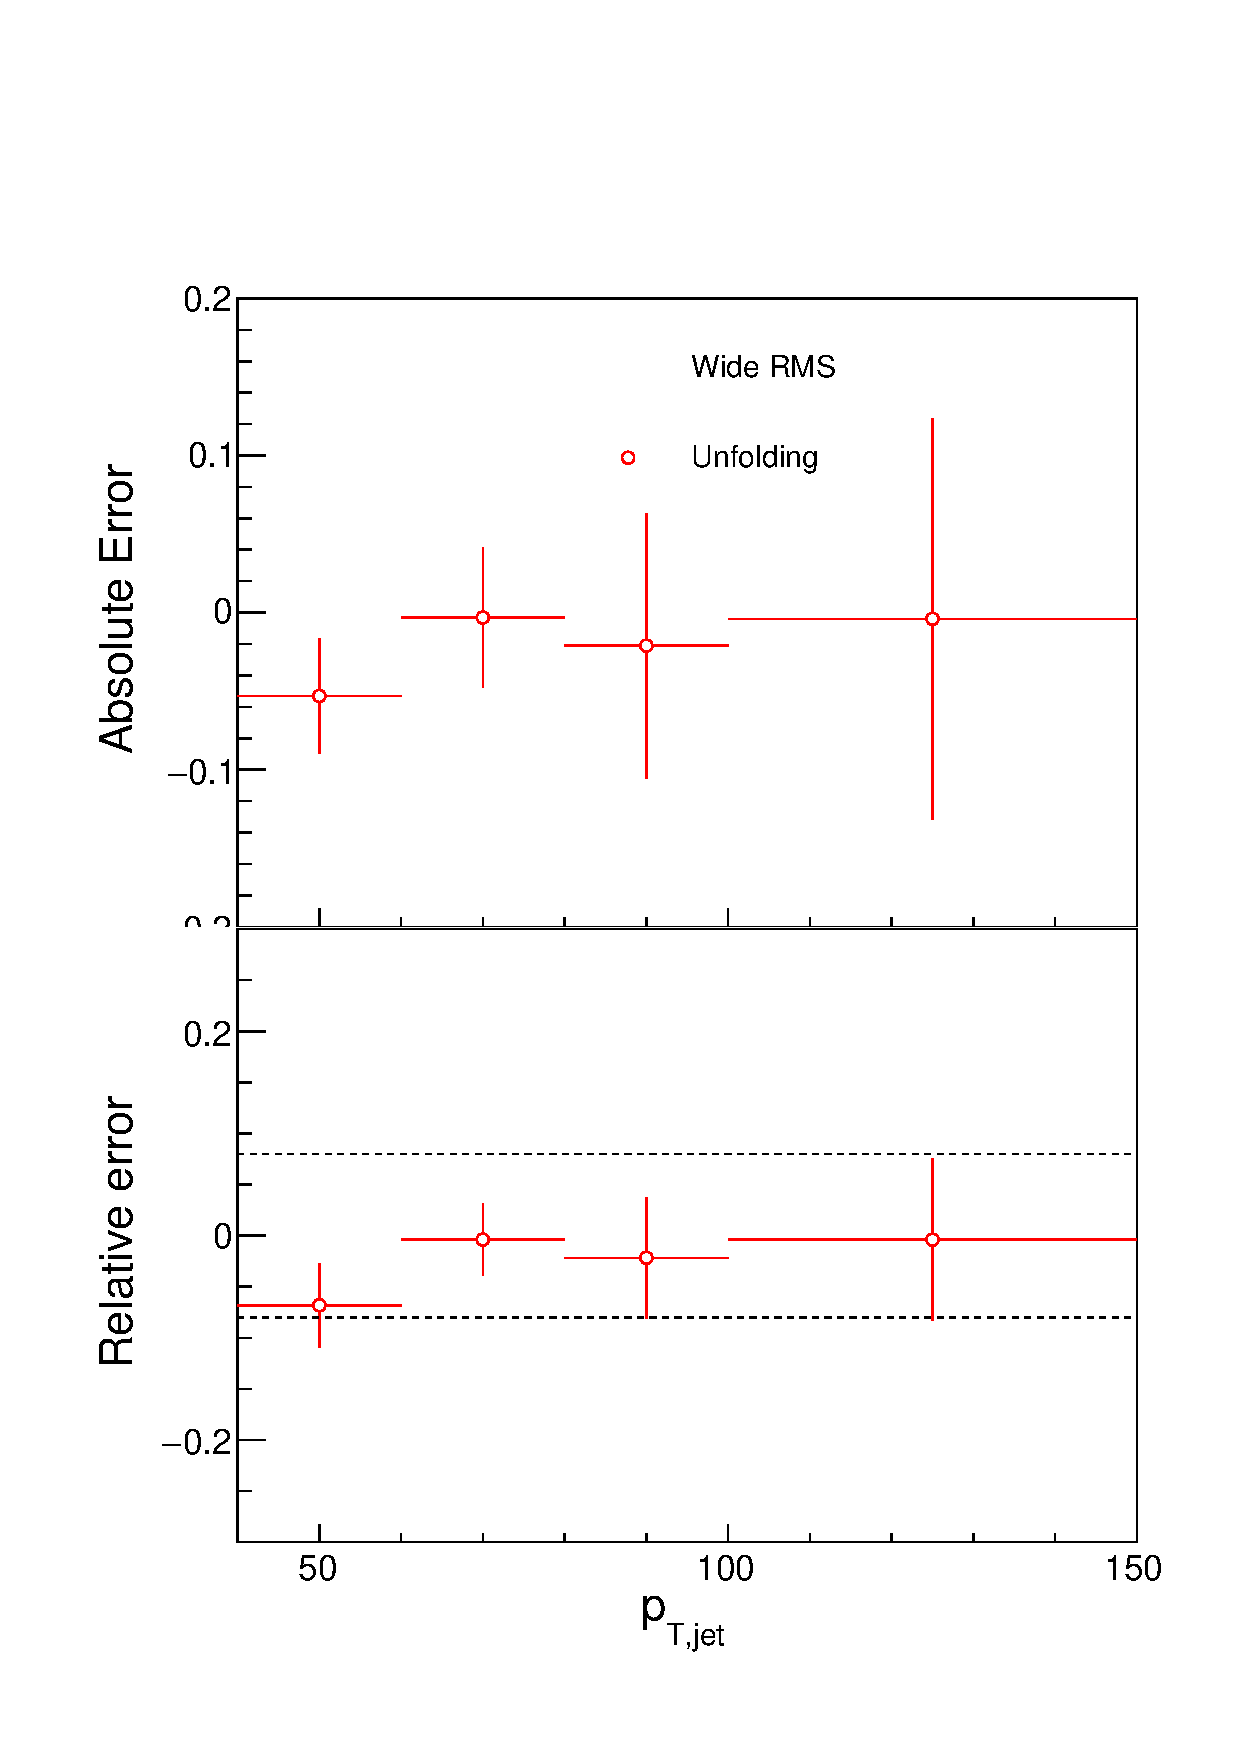
\includegraphics[width=0.95\textwidth]{results/SystematicErrors/SystematicErrorsGammaRMS_UnfNFin00JetPt08_linx_data}
\end{subfigure}
\begin{subfigure}{0.44\textwidth}
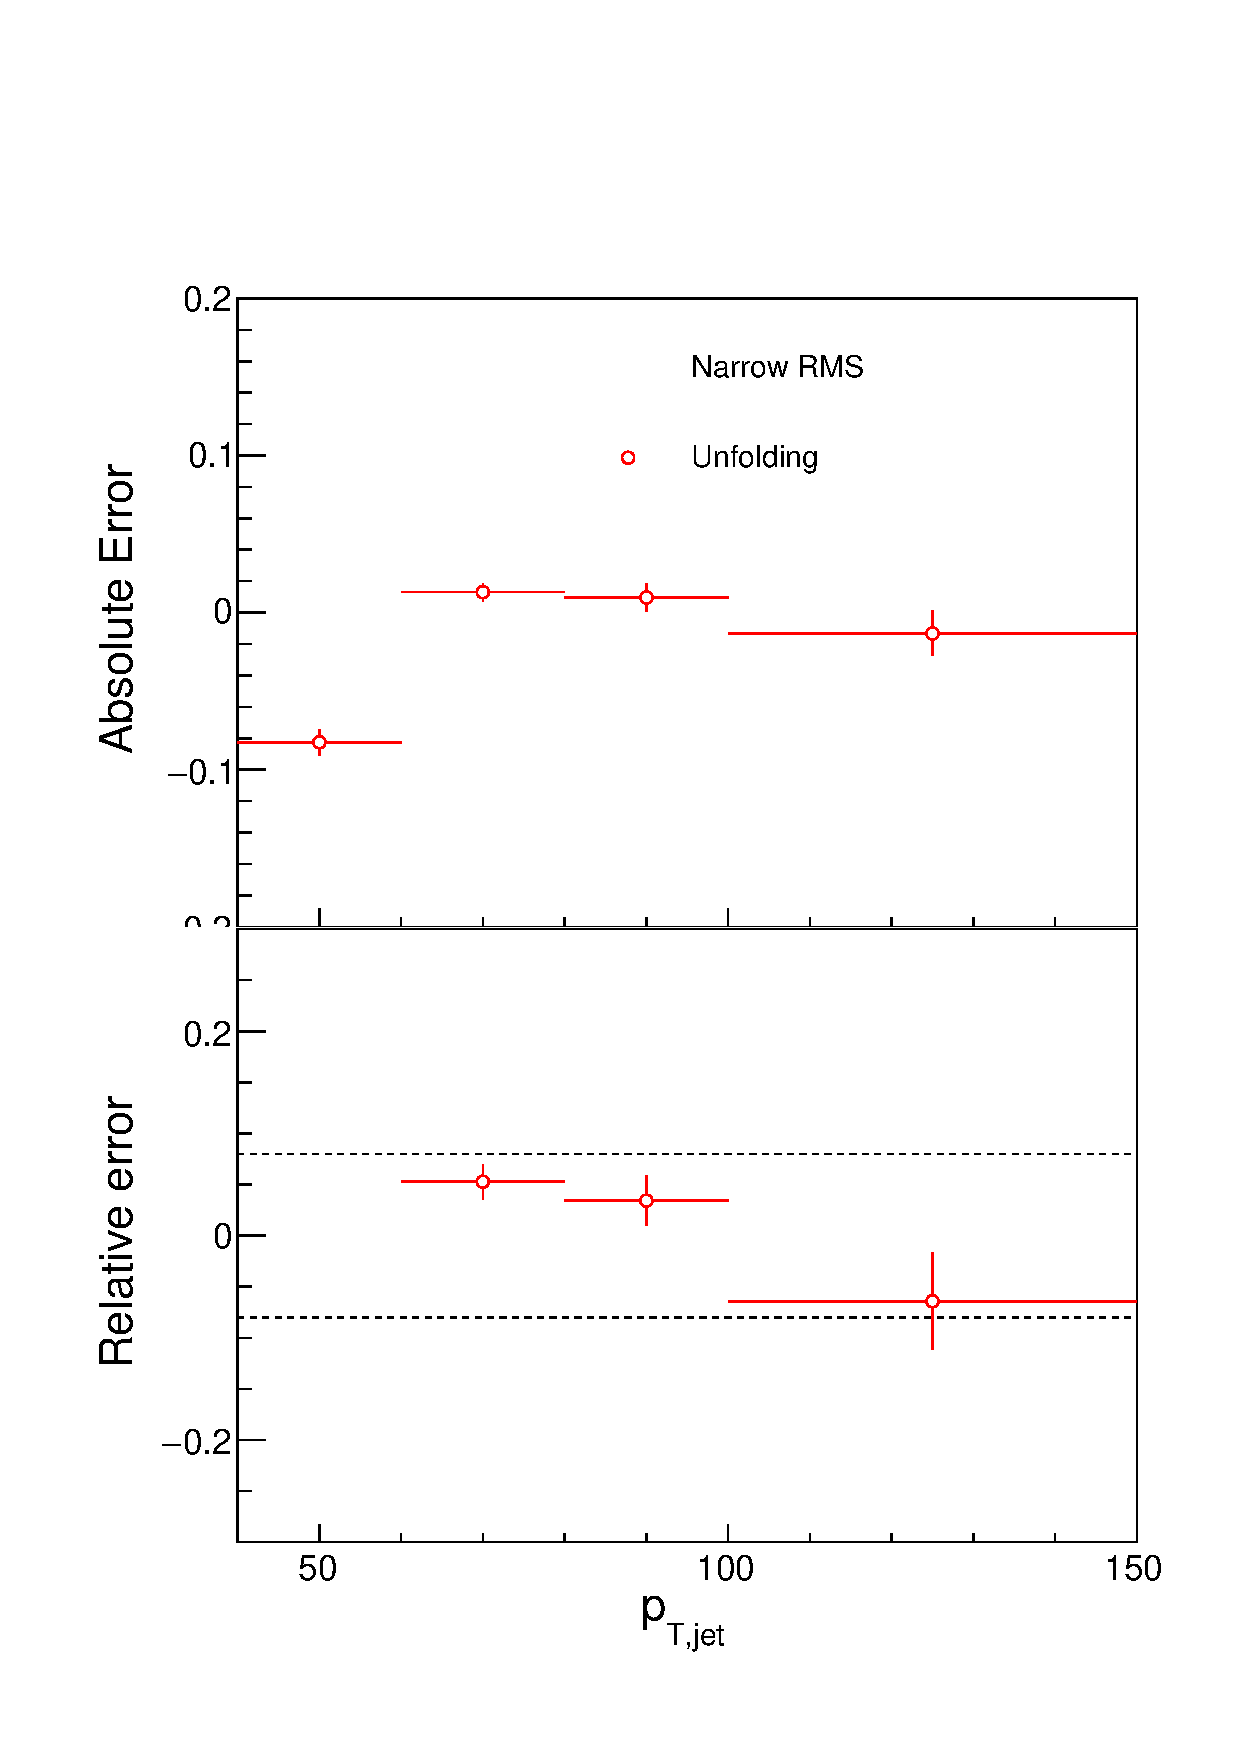
\includegraphics[width=0.95\textwidth]{results/SystematicErrors/SystematicErrorsGausRMS_UnfNFin00JetPt08_linx_data}
\end{subfigure}
\caption{Differences between Bayesian and SVD unfolding in the resulting RMS values}
\label{fig:systunf}
\end{figure}

Several other systematic checks were performed with the Bayesian unfolding procedure. They are described in the following sections. As these are small compared to the main uncertainty they are not included separately.
 
  
\subsubsection{Effect of number of iterations}
\label{}
The iterative unfolding algorithm permits the change of number of iterations. The unfolding procedure was carried out using different numbers of iterations. The results from these different cases are shown in Figure~\ref{fig:iterations}. The results are compared to the default unfolding algorithm with 4 iterations. The difference in results between the different cases is mostly less than 2.5\%.
\begin{figure}
\centering
%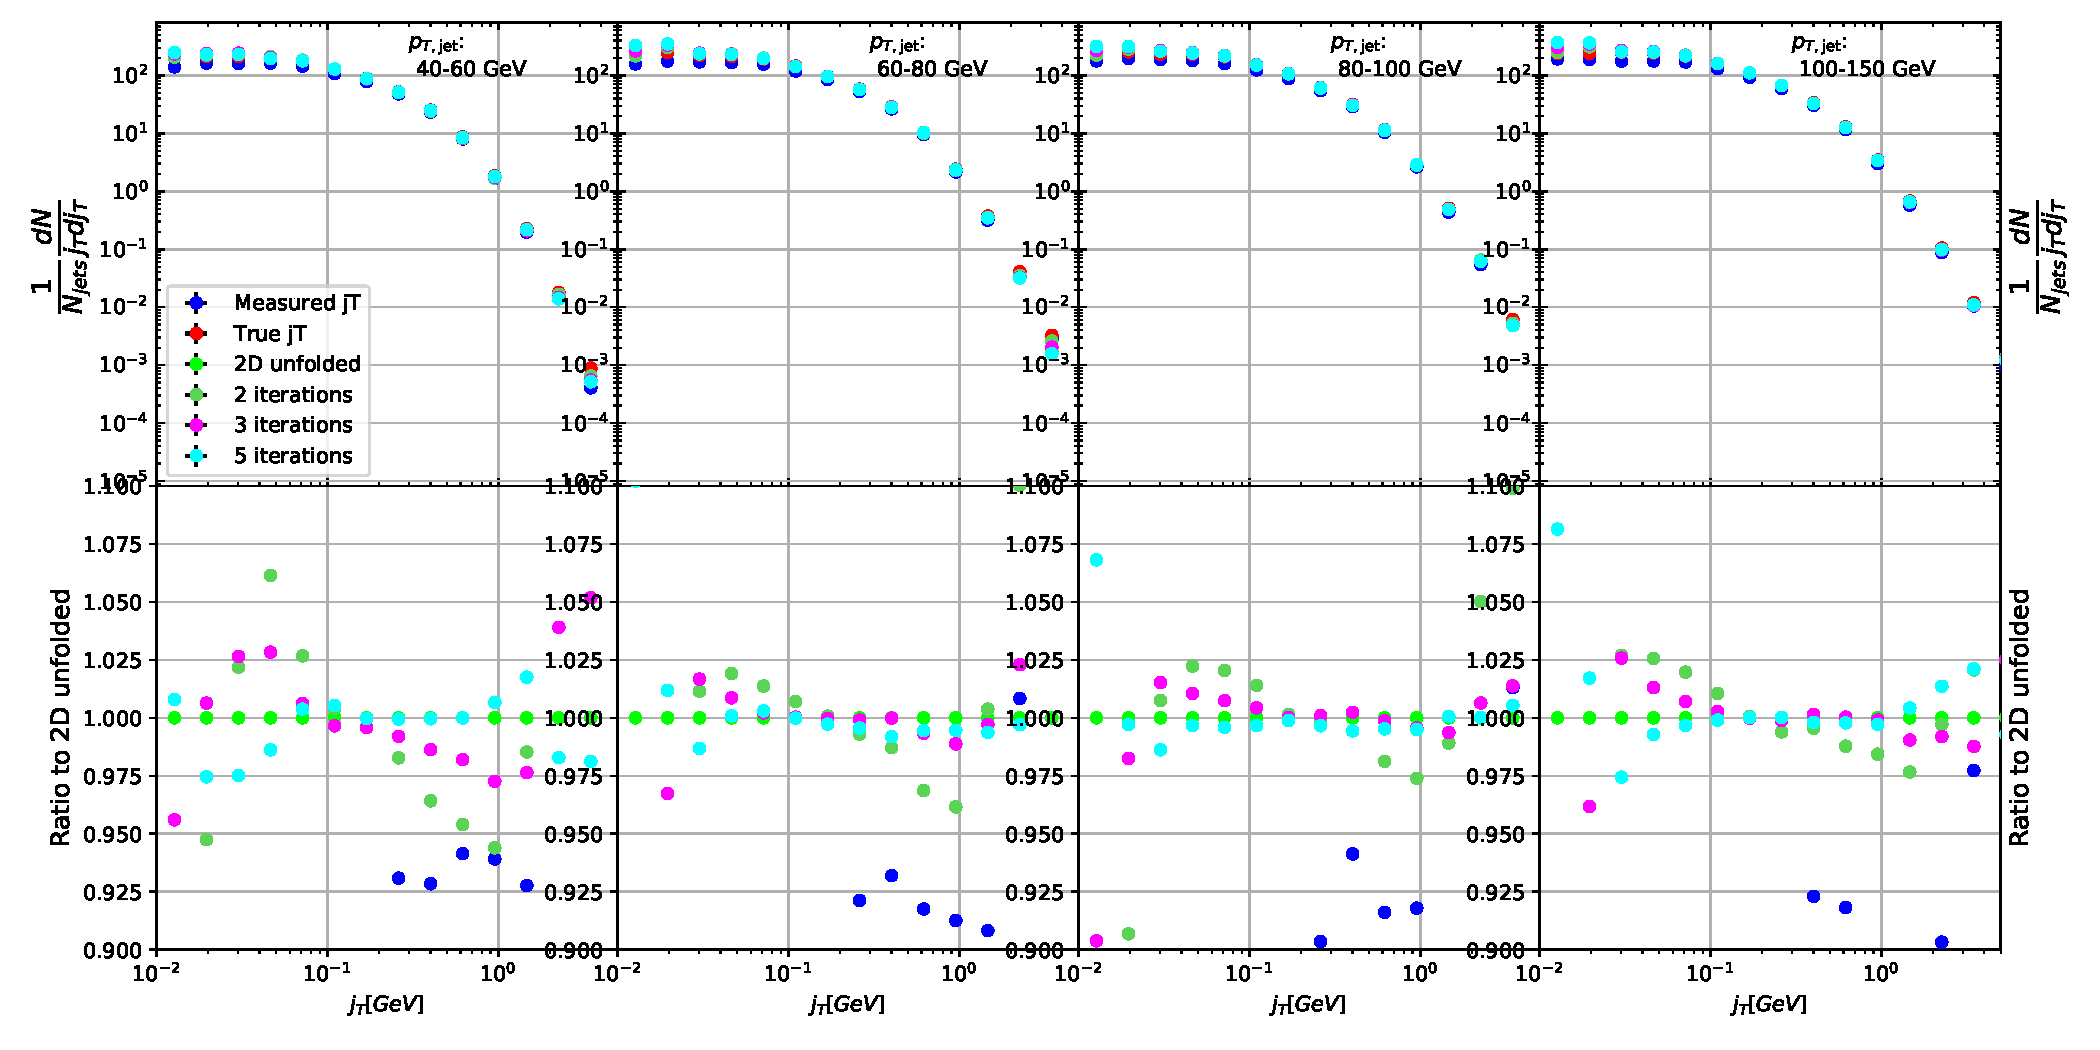
\includegraphics[width=0.99\textwidth]{figures/systematics/IterationsComparison.pdf}
\begin{subfigure}{0.44\textwidth}
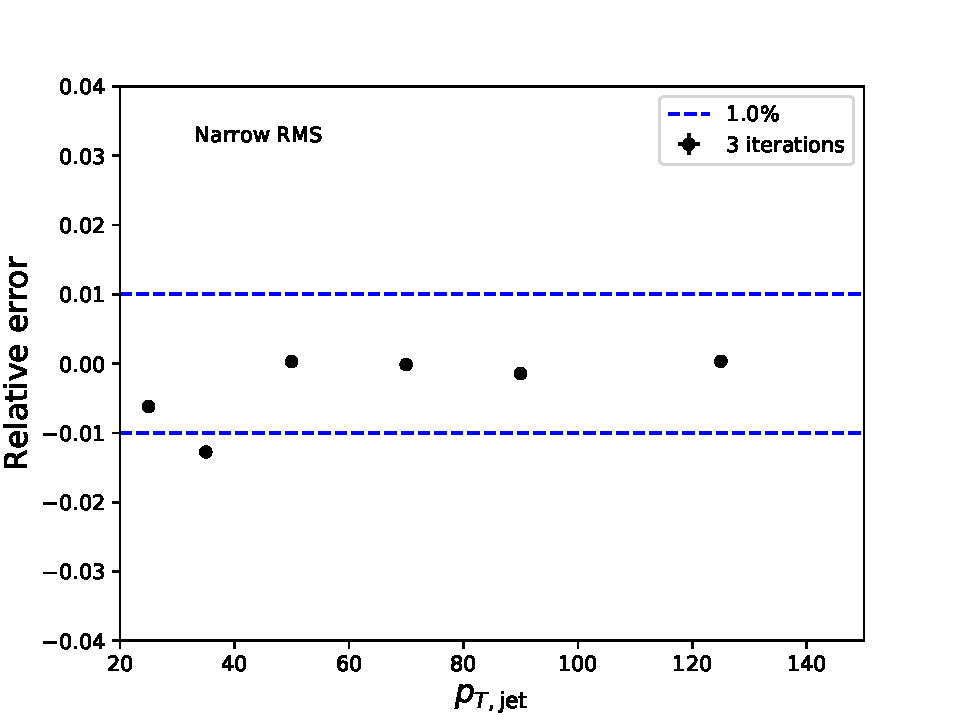
\includegraphics[width=0.95\textwidth]{figures/systematics/SystematicErrorsGausRMS_iterations.pdf}
\end{subfigure}
\begin{subfigure}{0.44\textwidth}
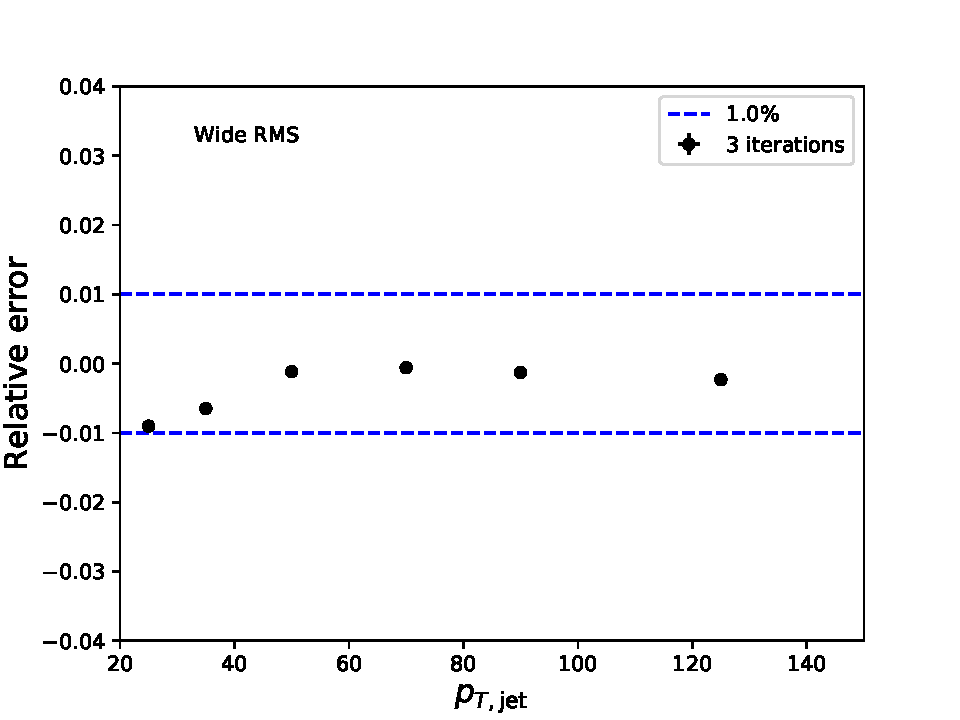
\includegraphics[width=0.95\textwidth]{figures/systematics/SystematicErrorsGammaRMS_iterations.pdf}
\end{subfigure}
\caption{Unfolding with different number of iterations}
\label{fig:iterations}
\end{figure}

\subsubsection{Effect of different prior}
\label{sec:prior}
The iterative algorithm requires a prior estimate of the shape of the distribution. As a default prior the truth (particle level) distribution is used. To test the effect of changing the prior we instead use the unfolded $\jt{}$ distribution as prior. The results are compared to the unfolding algorithm with the default prior. This is shown in Figure~\ref{fig:prior} The difference in results between the different cases is mostly less than 2.5\%. 

\begin{figure}
\centering
\begin{subfigure}{0.44\textwidth}
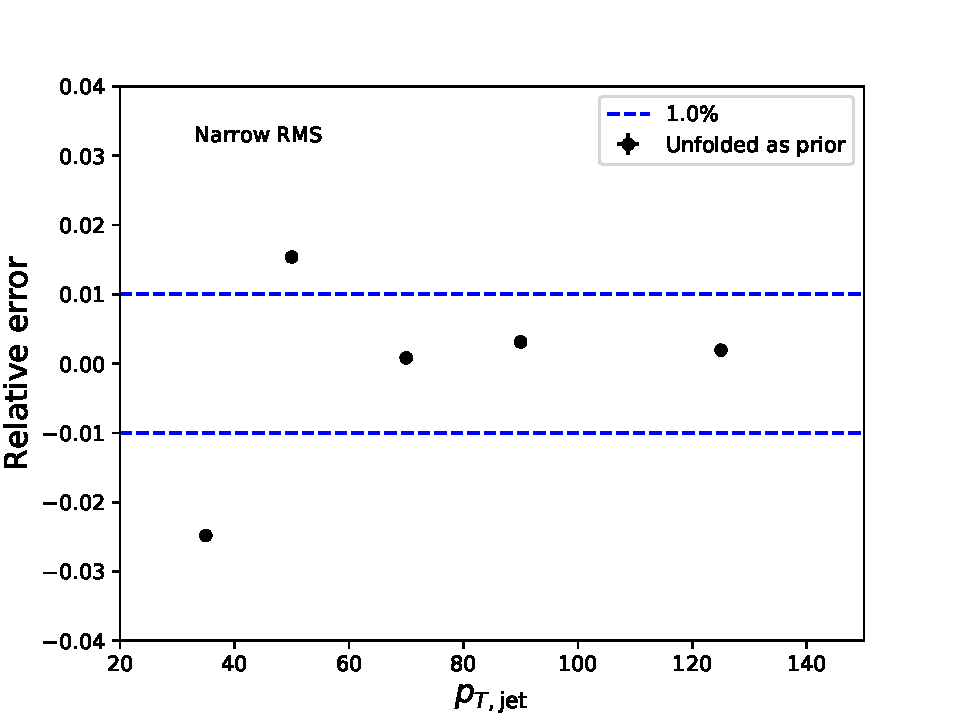
\includegraphics[width=0.95\textwidth]{figures/systematics/SystematicErrorsGausRMS_prior.pdf}
\end{subfigure}
\begin{subfigure}{0.44\textwidth}
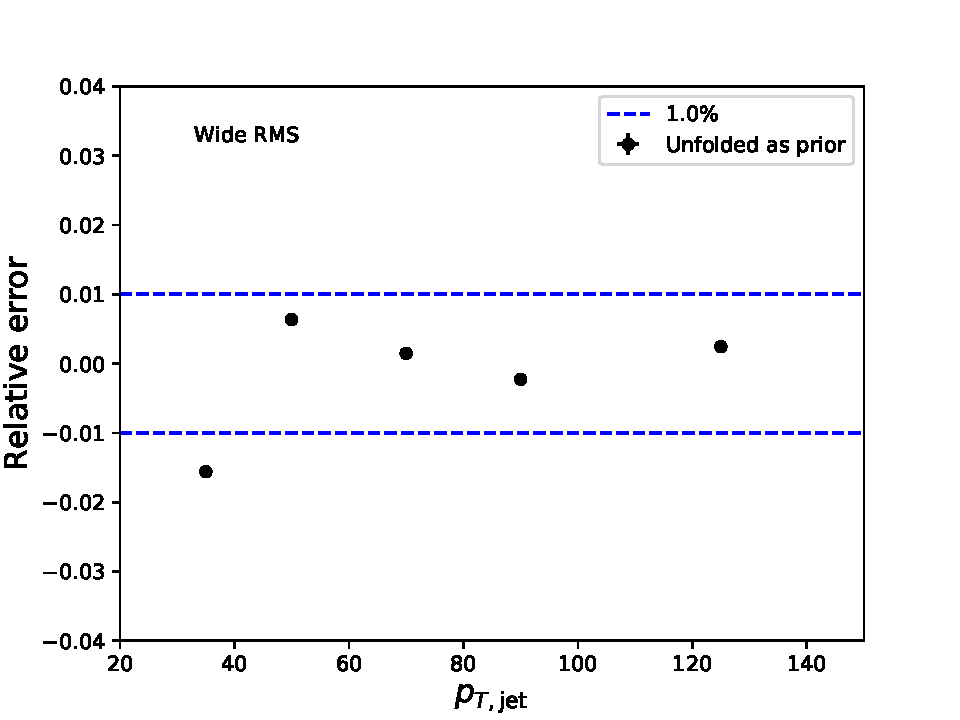
\includegraphics[width=0.95\textwidth]{figures/systematics/SystematicErrorsGammaRMS_prior.pdf}
\end{subfigure}
\caption{Effect of changing prior from true distribution in \pythia~to the unfolded distribution}
\label{fig:prior}
\end{figure}

\subsubsection{Effect of \texorpdfstring{$\pt{}$}{pT} truncation}
\label{sec:truncation}
As an additional check the unfolding is carried out with different $\pt{,jet}$ truncation values. By default the full range of $\pt{,jet} > 5 \gev$ is used. We test the unfolding by only using the response matrix for $\pt{,jet} > \unit[10]{\gev}$. The results of this test are shown in Figure~\ref{fig:truncation}. The effects are strongest in the lower $\pt{,jet}$ bins. Also in this case the difference is less than \unit[2.5]{\%} in all $\pt{,jet}$ bins.

\begin{figure}
\centering
\begin{subfigure}{0.45\textwidth}
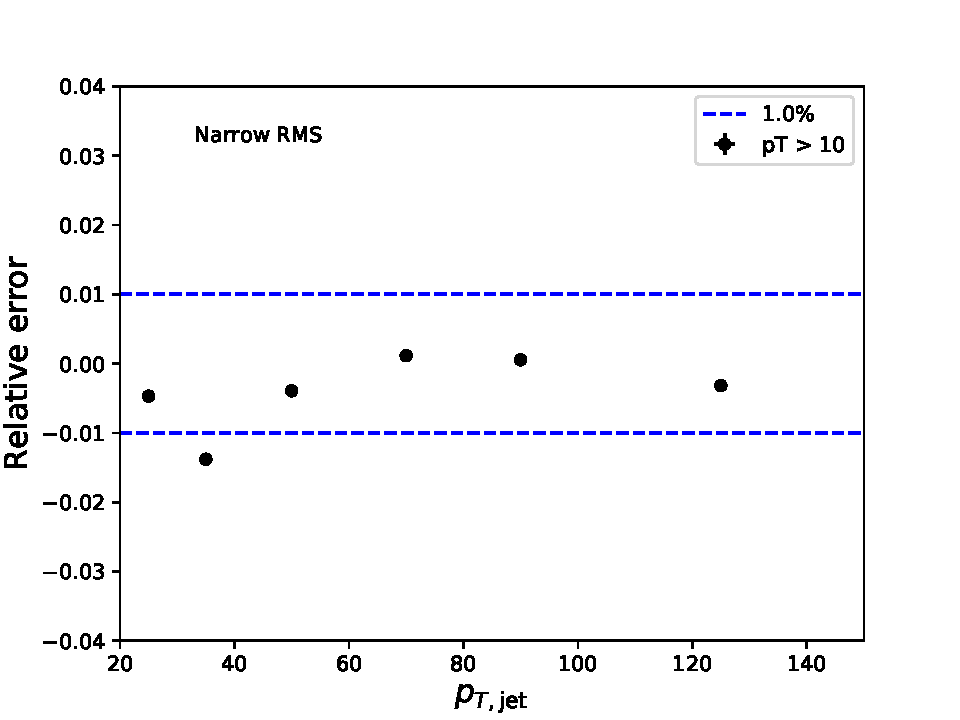
\includegraphics[width=0.95\textwidth]{figures/systematics/SystematicErrorsGausRMS_Truncation.pdf}
\end{subfigure}
\begin{subfigure}{0.45\textwidth}
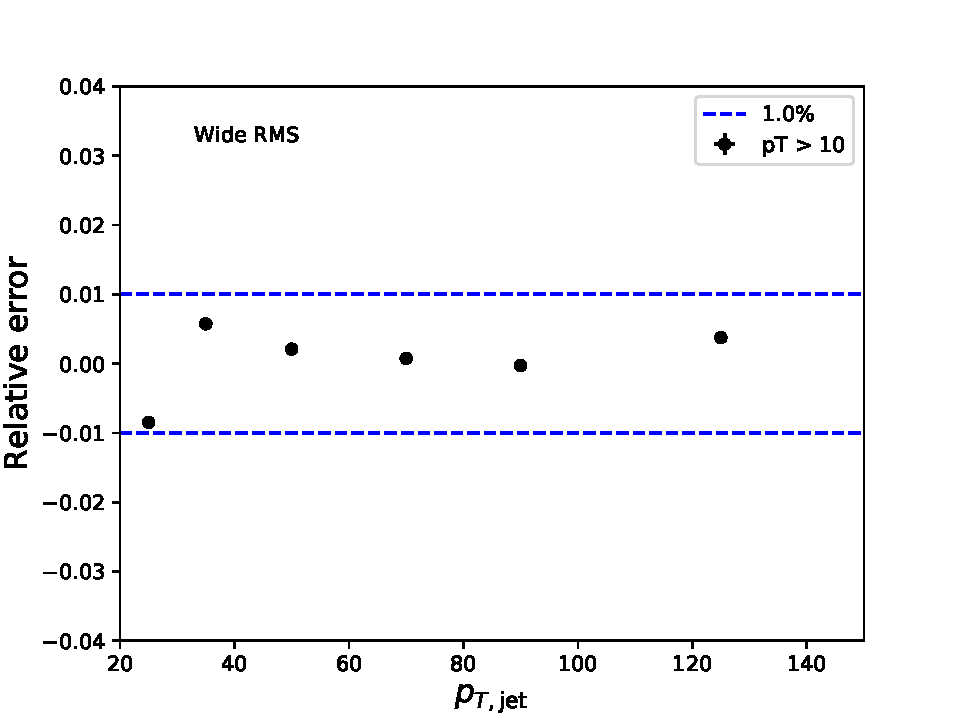
\includegraphics[width=0.95\textwidth]{figures/systematics/SystematicErrorsGammaRMS_Truncation.pdf}
\end{subfigure}
%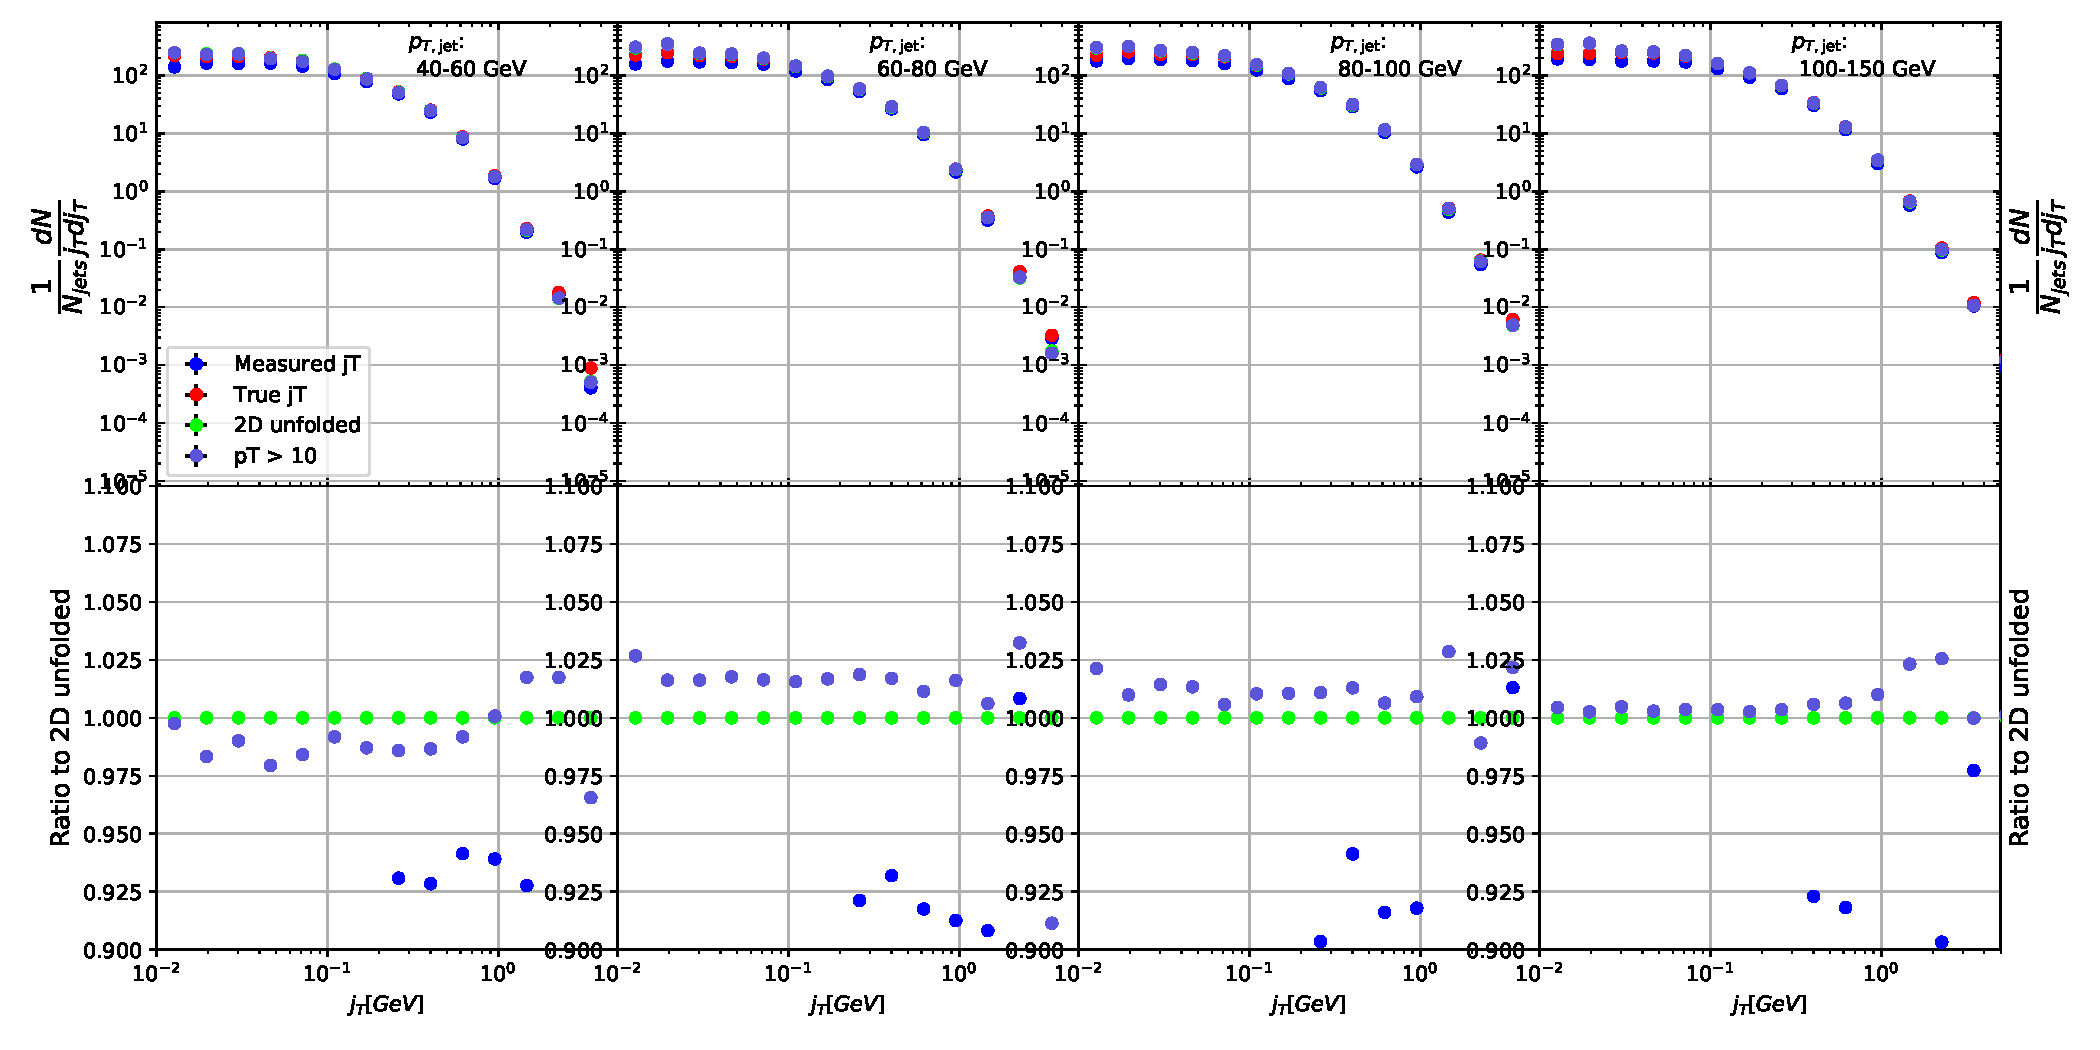
\includegraphics[width=0.99\textwidth]{figures/systematics/PtCutComparison10.pdf}
\caption{Effect of changing minimum jet $\pt{}$ used in unfolding from 5 to 10 \gev}
\label{fig:truncation}
\end{figure}

\subsection{Tracking}
Systematic effects originating from uncertainty in the tracking efficiency are estimated through a \pythia~simulation, where an artificial inefficiency of 3\% is introduced i.e. 3 \% of tracks are randomly removed from each event. The effect of this artificial inefficiency is shown in Figure~\ref{fig:systtrack2}. The systematic uncertainties assigned to tracking efficiency are \unit[4]{\%} for the narrow component and \unit[5]{\%} for the wide component. 

\begin{figure}
\centering
\begin{subfigure}{0.45\textwidth}
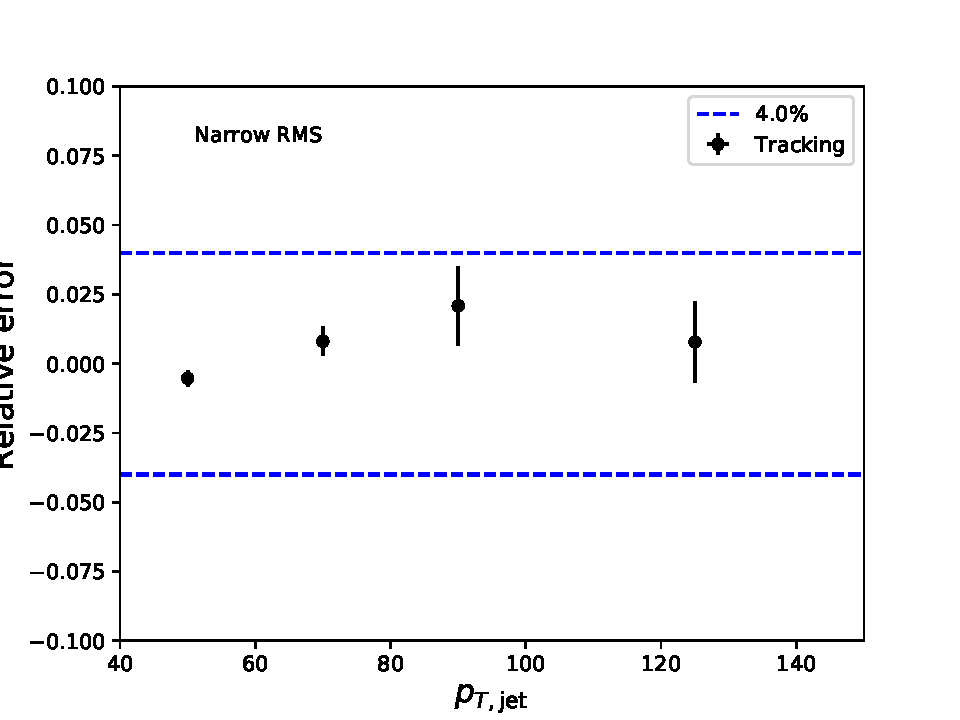
\includegraphics[width=0.95\textwidth]{figures/systematics/SystematicErrorsGausRMS_Tracking.pdf}
\end{subfigure}
\begin{subfigure}{0.45\textwidth}
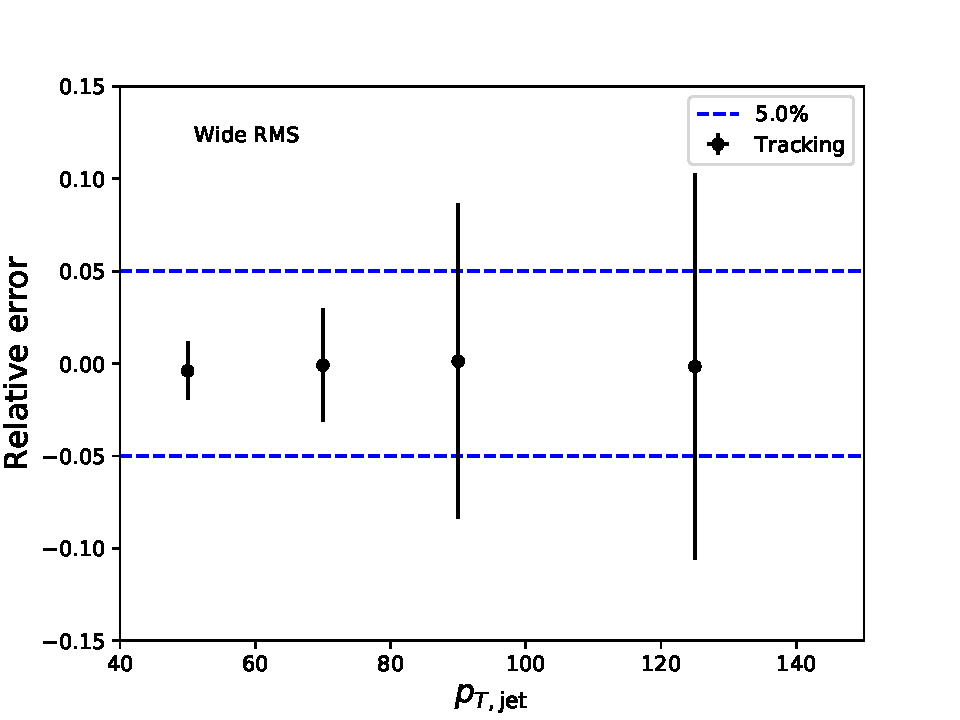
\includegraphics[width=0.95\textwidth]{figures/systematics/SystematicErrorsGammaRMS_Tracking.pdf}
\end{subfigure}
\caption{Relative systematic uncertainties resulting from uncertainty in tracking efficiency}
\label{fig:systtrack2}
\end{figure}

\subsection{EMCal clusters}
The analysis uses EMCal clusters only in the reconstruction of jets. Thus the only way uncertainty in EMCal performance can affect the results is through modification of jet momentum or axis.
  
Uncertainty related to the EMCal energy scale was estimated by scaling cluster energies up and down by 2 \% in a PYTHIA particle level simulation. Similarly the jet momentum was scaled by $\pm 2\%$ when determining the jet $\pt{}$ bin. In this analysis EMCal is used only in jet reconstruction, not for calculating $\jt{}$. The only ways EMCal uncertainty can affect the analysis are changes in jet energy and jet axis. Jet axis shouldn't significantly change, so the main contribution should be changes in jet $\pt{}$ bin.

The resulting differences in the inclusive $\jt{}$ distributions are shown in Figure~\ref{fig:systemcal}. Qualitatively the effect of scaling cluster energies is the same as scaling the jet energies.

Like in the previous cases fits are performed for the unscaled case and for cases with $\pm \unit[2]{\%}$ scaling. The resulting systematic uncertainties are shown in Figure~\ref{fig:systemcal2}. The uncertainty is taken to be 1\% for both components.

\begin{figure}
\centering
\begin{subfigure}{0.90\textwidth}
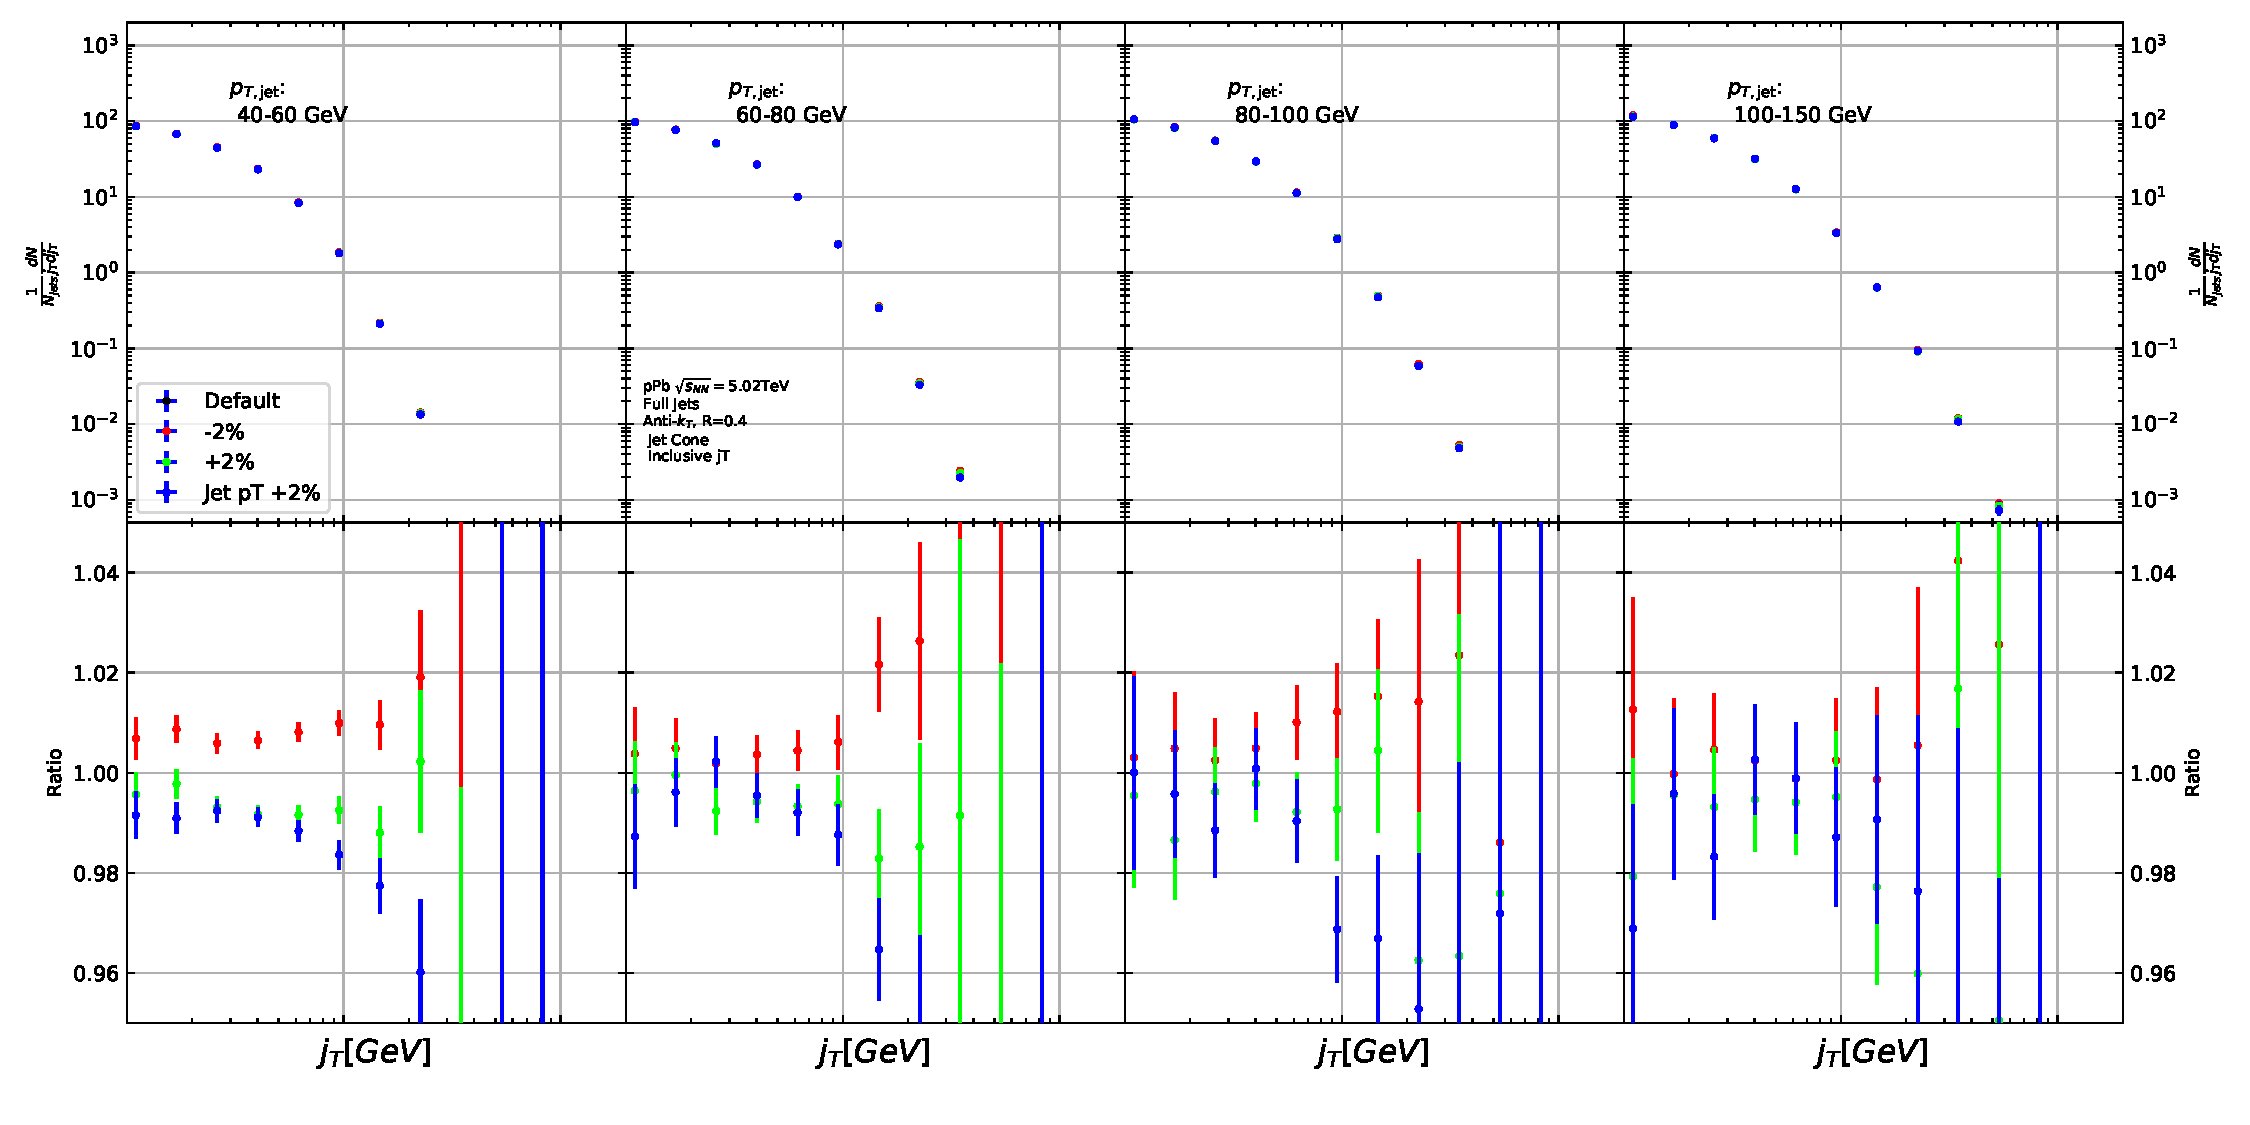
\includegraphics[width=0.95\textwidth]{figures/systematics/HadCorrComparisonJetPt4To8.pdf}
\end{subfigure}
%\begin{subfigure}{0.24\textwidth}
%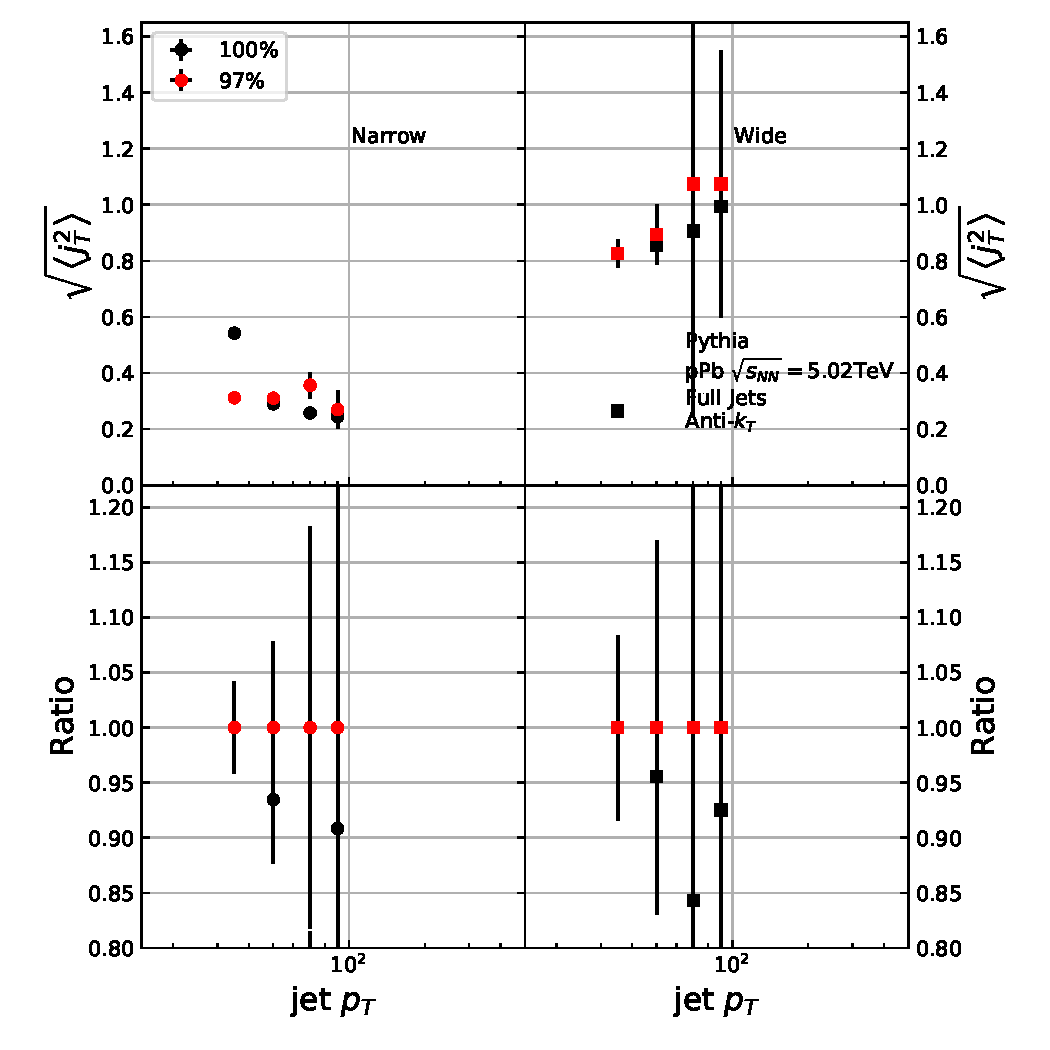
\includegraphics[width=0.95\textwidth]{RooUnfold/PythonFigures/TrackingSystematicsRMS.pdf}
%\end{subfigure}
\caption{Results from PYTHIA simulations with Cluster energies scaled up and down by 2 \%. Additionally jet momenta were scaled by 2 \% when determining the jet $\pt{}$ bin.}
\label{fig:systemcal}
\end{figure}

\begin{figure}
\centering
\begin{subfigure}{0.45\textwidth}
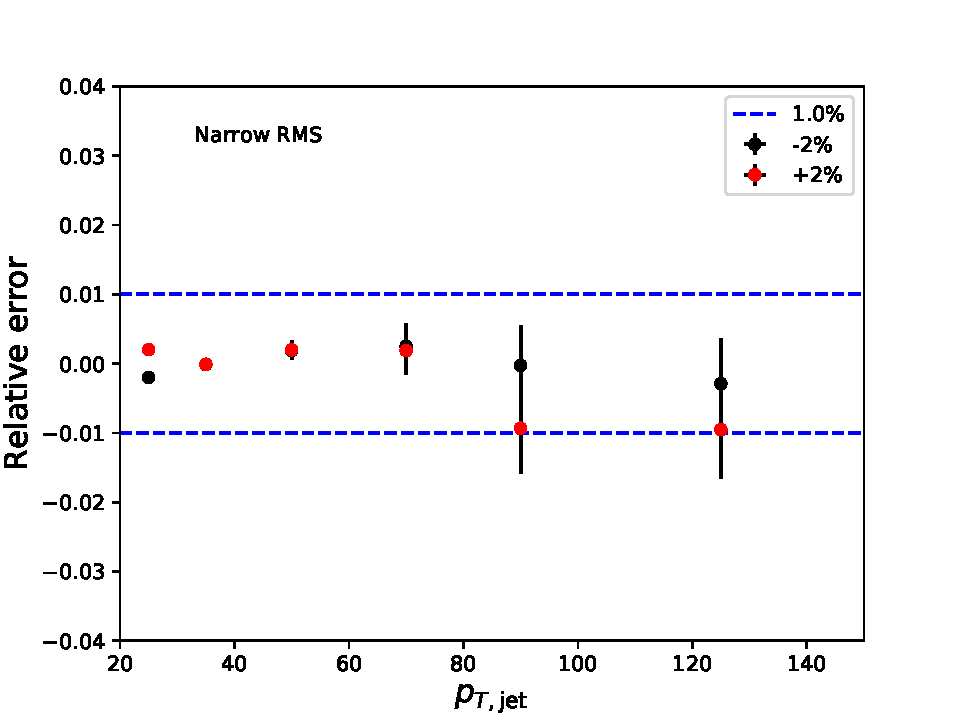
\includegraphics[width=0.95\textwidth]{figures/systematics/SystematicErrorsGausRMS_Emcal.pdf}
\end{subfigure}
\begin{subfigure}{0.45\textwidth}
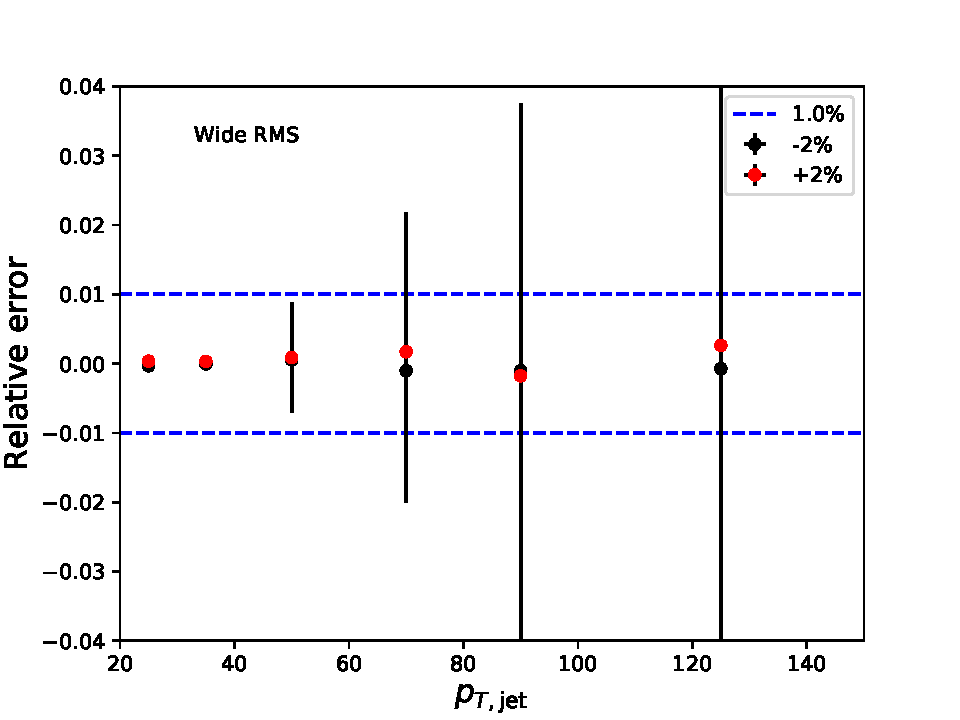
\includegraphics[width=0.95\textwidth]{figures/systematics/SystematicErrorsGammaRMS_Emcal.pdf}
\end{subfigure}
\caption{Relative systematic uncertainties resulting from cluster energy uncertainty.}
\label{fig:systemcal2}
\end{figure}


\FloatBarrier
\subsection{Summary of systematic uncertainties}

The different source of the systematic uncertainty are considered as uncorrelated and the values of each source are summed in quadrature. Resulting systematic uncertainties are shown in Table~\ref{tab:systematics}. The different source of the systematic uncertainty are considered to be uncorrelated and are thus combined bin-by-bin in quadrature to get the total systematic uncertainties.  The resulting uncertainty is approximately 10~\% for the wide component RMS and 13~\% for the narrow component RMS. 

\begin{table}[htb]
\centering
\caption{Summary of systematic uncertainties}
\label{tab:systematics}
\begin{tabular}{ l | c | r }
  Systematic & Wide RMS & Narrow RMS \\
    \hline			
  Background & 5 \% & 9 \% \\
  Unfolding & 8 \% & 8 \% \\
  Tracking & 4 \% & 5 \% \\ 
  EMCal & 1 \% & 1 \% \\
  Total & 10 \% & 13\% \\
  \hline
  \end{tabular}
  \end{table}


%  
%\subsection{Additional checks}
%\subsubsection{Comparison between A and C side}
%In 2013 there were issues with tracking. To rule out effects on $\jt{}$ distributions a study was performed comparing $\jt{}$ distributions between A and C side. (In the \pPb configuration the proton beam is travelling from A to C) No systematic differences were observed. Figure~\ref{fig:AC} shows the comparison between inclusive distributions between the different sides, both for minimum bias and EMCal triggered datasets.
%
%\begin{figure}
%\centering
%\begin{subfigure}{0.95\textwidth}
%%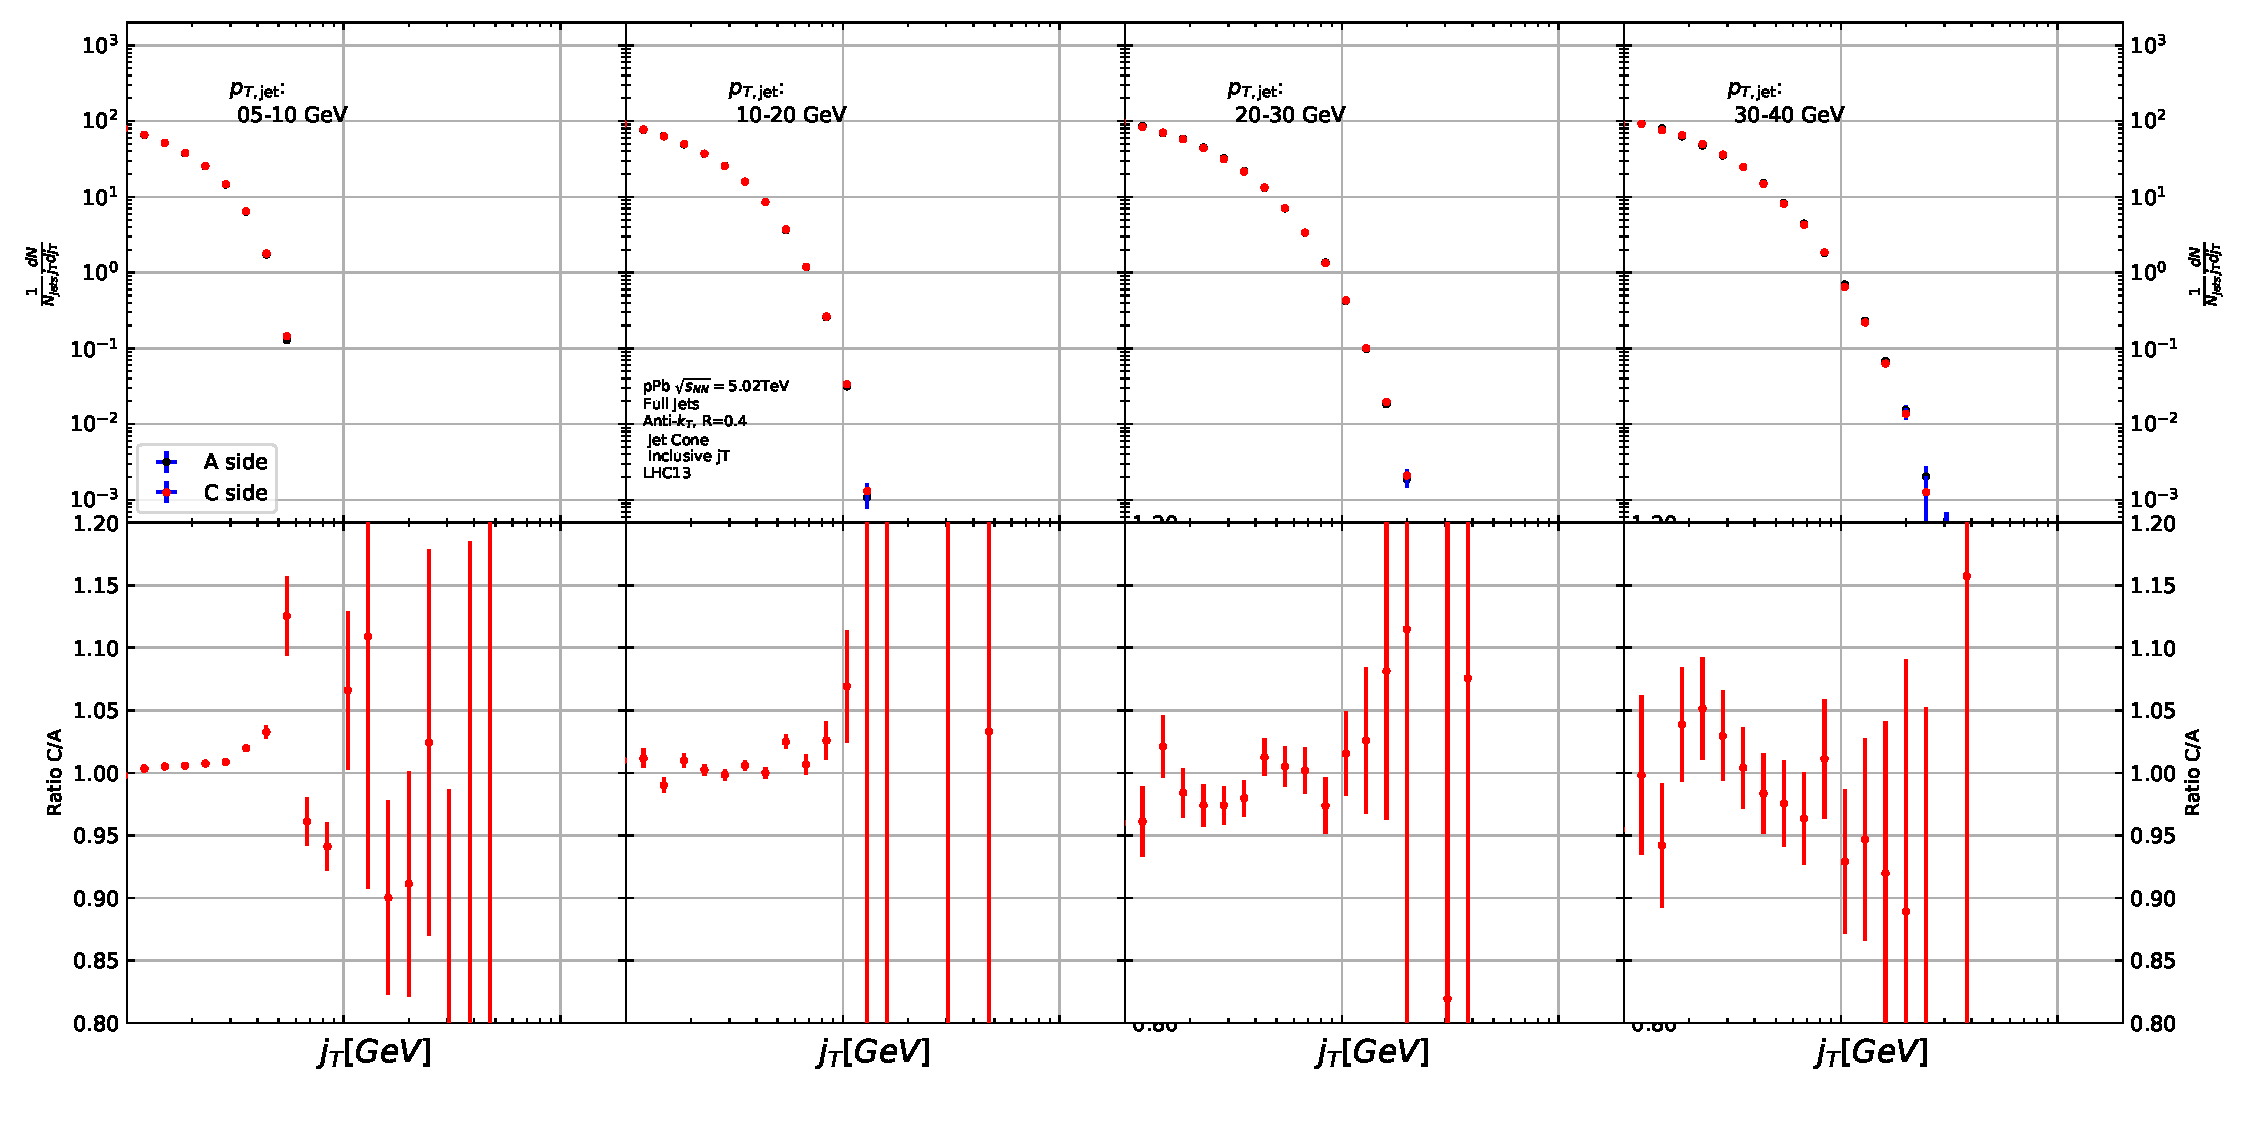
\includegraphics[width=\textwidth]{pics/ACsideComparison/ACsideJetConeJtInclusivePtFrom0To4LHC13.pdf}
%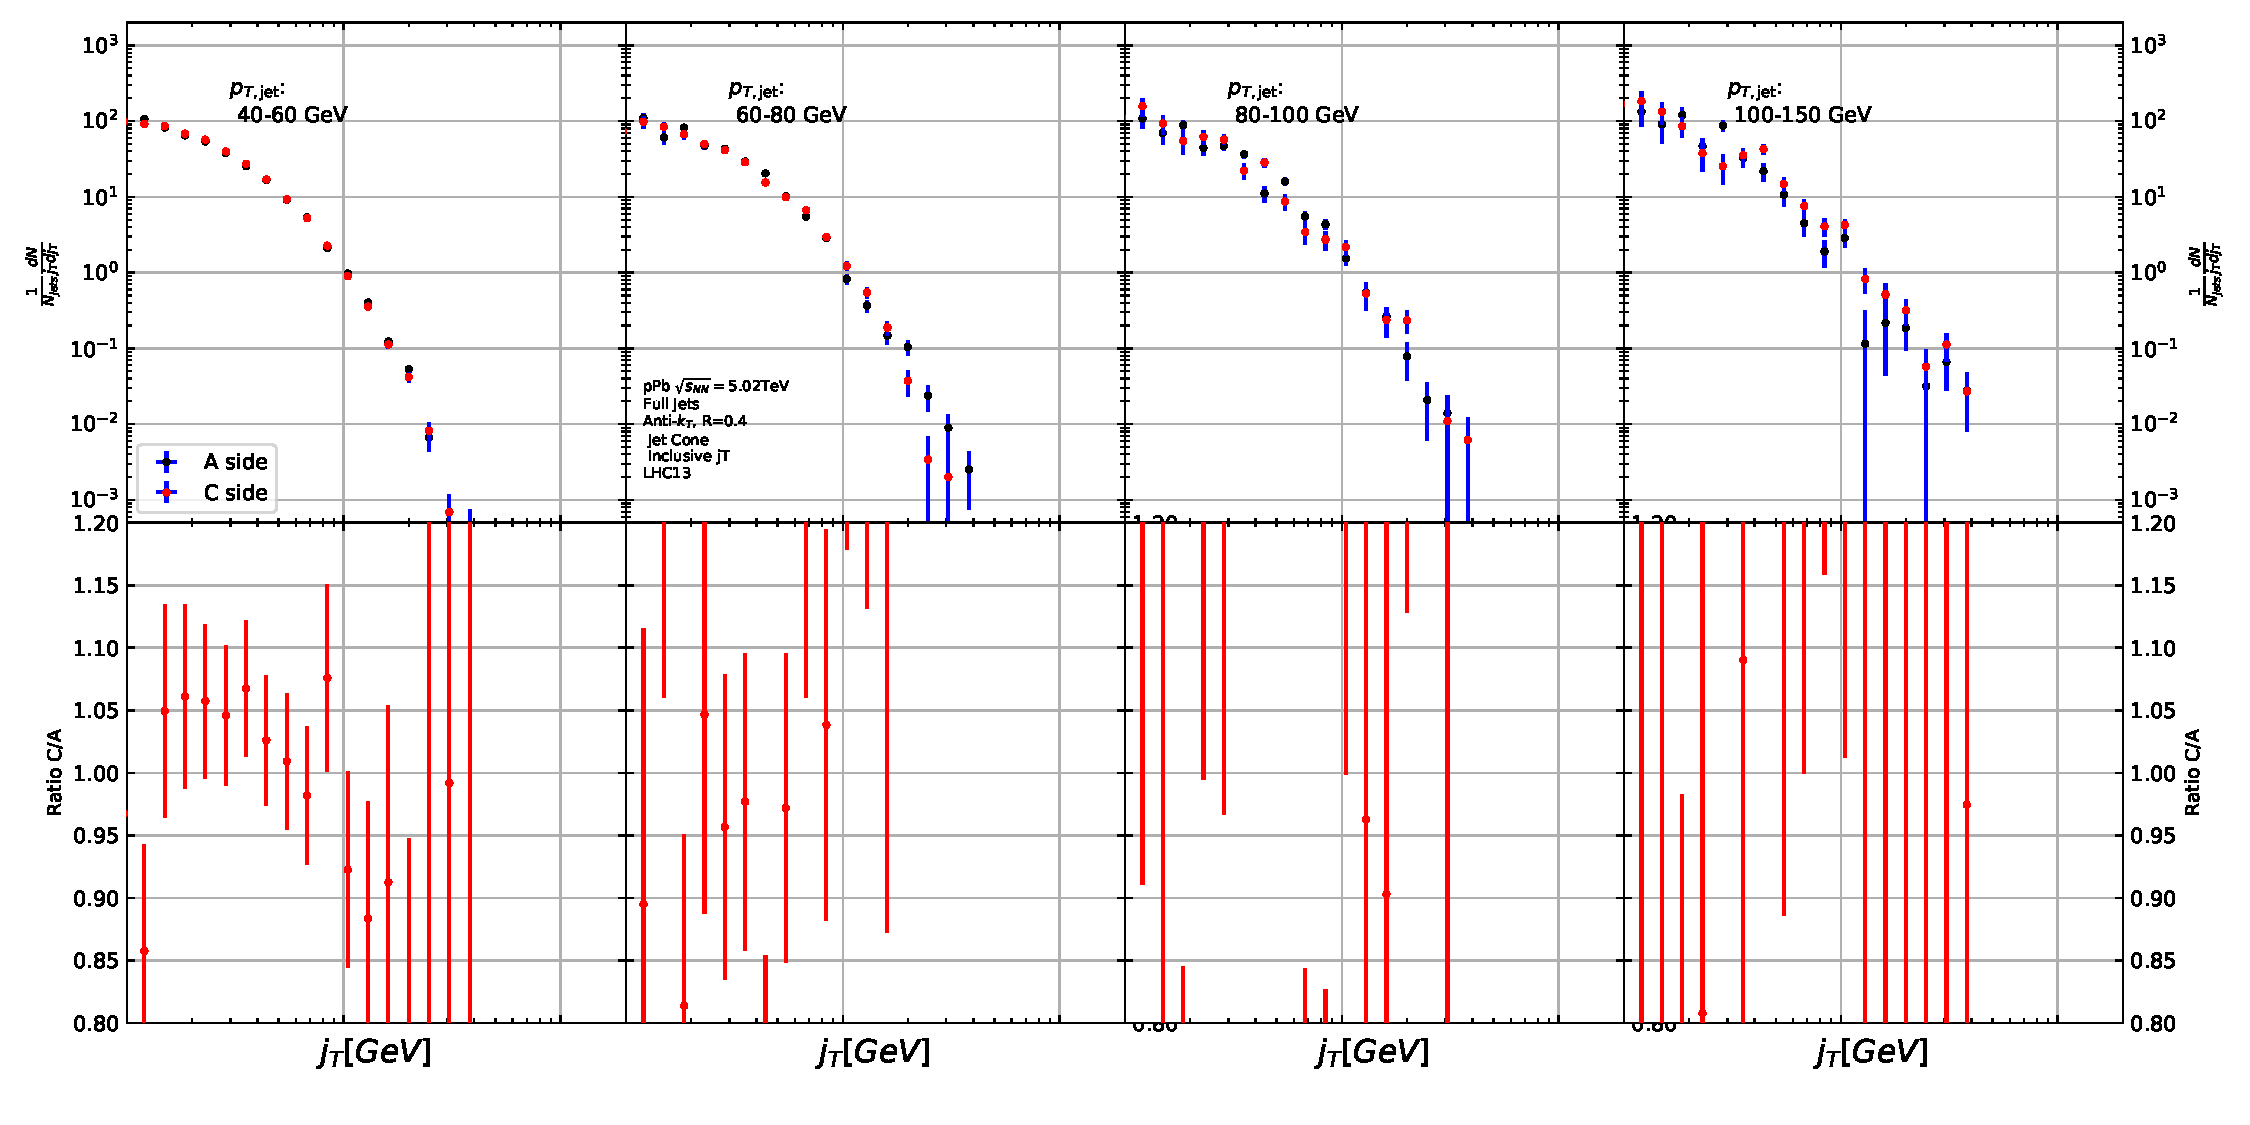
\includegraphics[width=\textwidth]{pics/ACsideComparison/ACsideJetConeJtInclusivePtFrom4To8LHC13.pdf}
%\includegraphics[width=\textwidth]{pics/ACsideComparison/ACsideJetConeJtInclusivePtFrom4To8LHC13EMCal.pdf}
%%Tag 20170810 python2.7 Python/DrawSignal.py legotrain_CF_pPb-1053_20170223-2002_LHC13bcde.root
%\end{subfigure}
%\caption{Comparison of inclusive $\jt{}$ distributions between A and C side for minimum bias and EMCal triggered data.}
%\label{fig:AC}
%\end{figure}

